\PassOptionsToPackage{table}{xcolor}
\documentclass[9pt, aspectratio=169]{beamer}
% \documentclass[10pt]{beamer}
\usepackage[utf8]{inputenc}
\usepackage[T1]{fontenc}


\usepackage[table]{xcolor}
\usepackage[backend=biber, style=authoryear]{biblatex}
\addbibresource{local_references.bib}

%\usepackage{lmodern}
\usepackage{amsfonts,amssymb,amsmath}
\usetheme{Frankfurt}
% \useoutertheme[subsection=true]{miniframes}

% \useoutertheme[subsection=true]{miniframes}
\makeatletter
\let\beamer@writeslidentry@miniframeson=\beamer@writeslidentry
\def\beamer@writeslidentry@miniframesoff{%
  \expandafter\beamer@ifempty\expandafter{\beamer@framestartpage}{}% does not happen normally
  {%else
    % removed \addtocontents commands
    \clearpage\beamer@notesactions%
  }
}
\newcommand*{\miniframeson}{\let\beamer@writeslidentry=\beamer@writeslidentry@miniframeson}
\newcommand*{\miniframesoff}{\let\beamer@writeslidentry=\beamer@writeslidentry@miniframesoff}
\makeatother

\usepackage{multirow}
\usepackage{fontawesome5}

\usepackage{csquotes}
\usepackage[english]{babel}
\usepackage{csquotes}
\usepackage{setspace}
\usepackage{arydshln}

\usepackage{colortbl}
\usepackage{tabularx}
\renewcommand\tabularxcolumn[1]{m{#1}}

% --- Tickz
\usepackage{physics}
\usepackage{amsmath}
\usepackage{tikz}
\usepackage{mathdots}
\usepackage{yhmath}
\usepackage{cancel}
\usepackage{color}
\usepackage{siunitx}
\usepackage{array}
\usepackage{multirow}
\usepackage{amssymb}
\usepackage{gensymb}
\usepackage{tabularx}
\usepackage{extarrows}
\usepackage{booktabs}
\usetikzlibrary{fadings}
\usetikzlibrary{patterns}
\usetikzlibrary{shadows.blur}
\usetikzlibrary{shapes}

% ---------

\usepackage{booktabs}
\usepackage{setspace}
\usepackage{amssymb}
\usepackage{adjustbox}
\usepackage{pifont}
\usepackage[inkscapeformat=png]{svg}
\usepackage{graphicx}
\usepackage{times}
\setbeamertemplate{caption}[numbered]
% % \setbeamertemplate{bibliography item}{[\theenumiv]}

\setbeamerfont{bibliography item}{size=\tiny}
\setbeamerfont{bibliography entry author}{size=\tiny}
\setbeamerfont{bibliography entry title}{size=\tiny}
\setbeamerfont{bibliography entry location}{size=\tiny}
\setbeamerfont{bibliography entry note}{size=\tiny}

\setbeamerfont{frametitle}{size=\large}

\usepackage{caption}
\usepackage{float}
\usepackage{xcolor}
\usepackage{listings}
\usepackage{animate}
\usepackage{forest}

\definecolor{codegreen}{rgb}{0,0.6,0}
\definecolor{codegray}{rgb}{0.5,0.5,0.5}
\definecolor{codepurple}{rgb}{0.58,0,0.82}
\definecolor{backcolour}{rgb}{0.95,0.95,0.92}
 
\newcommand{\sensinterdit}{%
\tikz[baseline=-0.5ex]{
  \draw[red, line width=1pt, fill=red] (0,0) circle (0.8ex);
  \draw[white, line width=1pt] (-0.6ex,0) -- (0.6ex,0);
}}

\lstdefinestyle{mystyle}{
    backgroundcolor=\color{backcolour},   
    commentstyle=\color{codegreen},
    keywordstyle=\color{magenta},
    numberstyle=\tiny\color{codegray},
    stringstyle=\color{codepurple},
    basicstyle=\footnotesize,
    breakatwhitespace=false,         
    breaklines=true,                 
    captionpos=b,                    
    keepspaces=true,                 
    numbers=left,                    
    numbersep=5pt,                  
    showspaces=false,                
    showstringspaces=false,
    showtabs=false,                  
    tabsize=2
}
 
\lstset{style=mystyle}

\usepackage{ragged2e}
\setbeamercolor{section in foot}{fg=white,bg=darkorange}
\setbeamercolor{subsection in foot}{fg=white,bg=darkorange}
\setbeamercolor{frametitle}{fg=white, bg=darkorange}
\setbeamercolor{title}{fg=white, bg=darkorange}
\setbeamercolor{frame}{bg=darkorange}
\setbeamercolor{block title}{bg=darkorange,fg=white}

\setbeamercolor{item}{fg=darkorange}

% \definecolor{darkorange}{rgb}{0.81, 0.52, 0.05}
\definecolor{darkorange}{rgb}{1,0.5,0}
\definecolor{darkorange2}{rgb}{1, 0.64, 0.2}
\definecolor{honeydew}{rgb}{1, 0.85, 0.45}


\newenvironment{variableblock}[3]{%
  \setbeamercolor{block body}{#2}
  \setbeamercolor{block title}{#3}
  \begin{block}{#1}}{\end{block}}

\newenvironment{prosblock}[1]{%
  % \setbeamercolor{block body}{bg=blue,fg=white}
  \setbeamercolor{block title}{bg=blue,fg=white}
  \begin{block}{#1}}{\end{block}}

\newenvironment{consblock}[1]{%
  % \setbeamercolor{block body}{bg=red,fg=white}
  \setbeamercolor{block title}{bg=red,fg=white}
  \begin{block}{#1}}{\end{block}}

\newcommand{\cmark}{\ding{51}}%
\newcommand{\xmark}{\ding{55}}%

\renewcommand{\arraystretch}{1.5}
\newcommand{\vcentered}[1]{\raisebox{-.5\height}{#1}}

% Please add the following required packages to your document preamble:
\usepackage{booktabs}
\usepackage{multirow}
\usepackage{colortbl}
% Beamer presentation requires \usepackage{colortbl} instead of \usepackage[table,xcdraw]{xcolor}

\usepackage{tabularray}\UseTblrLibrary{varwidth}
\usepackage{xcolor}
\def\BibTeX{{\rm B\kern-.05em{\sc i\kern-.025em b}\kern-.08em
    T\kern-.1667em\lower.7ex\hbox{E}\kern-.125emX}}
% \usepackage{cite}
\usepackage{amsmath}
\newcommand{\probP}{\text{I\kern-0.15em P}}
\usepackage{etoolbox}
\patchcmd{\thebibliography}{\section*{\refname}}{}{}{}

\setlength\tabcolsep{0.5pt}

\renewcommand{\arraystretch}{0.9}
\setlength{\tabcolsep}{2pt}

\usepackage{pgffor}
\usepackage[absolute,overlay]{textpos}
\setlength{\TPHorizModule}{1cm}
\setlength{\TPVertModule}{1cm}

\setbeamerfont{bibliography item}{size=\tiny}
\setbeamerfont{bibliography entry author}{size=\tiny}
\setbeamerfont{bibliography entry title}{size=\tiny}
\setbeamerfont{bibliography entry location}{size=\tiny}
\setbeamerfont{bibliography entry note}{size=\tiny}

\setbeamerfont{bibliography entry author}{shape=\upshape,series=\mdseries,size=\footnotesize}
\setbeamerfont{bibliography entry title}{shape=\slshape,series=\mdseries,size=\footnotesize}
\setbeamerfont{bibliography entry journal}{shape=\upshape,series=\mdseries,size=\footnotesize}
\setbeamerfont{bibliography entry note}{shape=\upshape,series=\mdseries,size=\footnotesize}

\renewcommand*{\bibfont}{\scriptsize}

\newenvironment<>{varblock}[2][.9\textwidth]{%
  \setlength{\textwidth}{#1}
  \begin{actionenv}#3%
    \def\insertblocktitle{#2}%
    \par%
    \usebeamertemplate{block begin}}
  {\par%
    \usebeamertemplate{block end}%
  \end{actionenv}}

\newenvironment<>{alertvarblock}[2][.9\textwidth]{%
  \setlength{\textwidth}{#1}%
  \begin{actionenv}#3%
    \begin{alertblock}{#2}%
}{%
    \end{alertblock}%
  \end{actionenv}%
}

% \setbeamertemplate{footline}[frame number]

\setbeamertemplate{footline}{
  \leavevmode%
  \hfill
  \usebeamercolor[fg]{page number in head/foot}%
  \scriptsize%
  \ifnum\value{framenumber}>52%
    Appendix \number\numexpr\value{framenumber}-52\relax/53%
  \else%
    \ifnum\value{framenumber}>41%
      %
    \else
      \number\numexpr\value{framenumber}\relax/41%
    \fi

  \fi%
  \hspace{1em}
}


\begin{document}

\author{
  {\Large \textbf{Julien Soulé}}
}

\title[On the Organization of a Cyber-Defense Multi-Agent System (AICA)]{\textbf{On the Organization of a Cyber-Defense Multi-Agent System}}

\subtitle{PhD Defense in Computer Science}

\date{

{ \tiny

\noindent \textbf{Jean-Paul Jamont}, Full Professor, Grenoble Alpes University -- PhD supervisor

\vspace{0.15cm}

\noindent \textbf{Michel Occello}, Full Professor, Grenoble Alpes University -- Co-supervisor

\vspace{0.15cm}

\noindent \textbf{Louis-Marie Traonouez}, PhD, Thales Land and Air Systems, BU IAS -- Industrial supervisor

\vspace{0.15cm}

\noindent \textbf{Paul Théron}, PhD, AICA IWG -- Scientific advisor\\[2em]
{\normalsize \textit{17 November 2025}}

}

}

\institute{{\small \textit{Laboratoire de Conception
        et d'Intégration des Systèmes, Valence, France\\
        Thales Land \& Air Systems, Rennes, France}}}

%\subject{}
\setbeamercovered{transparent}
\setbeamertemplate{navigation symbols}{}
\begin{frame}[plain]
  \vspace{0.5cm}
  \maketitle\vspace{-0.2cm}
  \begin{figure}[ht!]
    \centering

    \centering
    \begin{minipage}{0.25\textwidth}
      \centering
      \includesvg[height=0.4cm]{figures/thales_logo.svg}
    \end{minipage}\hfill
    \begin{minipage}{0.25\textwidth}
      \centering
      
\includegraphics[height=1.2cm]{figures/la-ruche_logo.png}
    \end{minipage}\hfill
    \begin{minipage}{0.25\textwidth}
      \centering
      
\includegraphics[height=0.6cm]{figures/lcis_logo.png}
    \end{minipage}\hfill
    \begin{minipage}{0.25\textwidth}
      \centering
      
\includegraphics[height=1cm]{figures/uga_logo.jpg}
    \end{minipage}

  \end{figure}


\end{frame}


\addtocounter{framenumber}{-1}

\section{Introduction}

% \AtBeginSection[]{
%   \begin{frame}
%     \frametitle{}
%     \tableofcontents[currentsection]
%   \end{frame}
% }

\begin{frame}{Introduction}{Background}

  \begin{columns}

    \begin{column}{0.7\textwidth}
      \begin{itemize}
        \item Increasing \textbf{attack surface}:
              \begin{itemize}
                \item IoT and cloud weaknesses\dots
                \item Time constraints, workload, and complexity\dots
                \item Jamming and communication disruption\dots
              \end{itemize}
      \end{itemize}
      $\Longrightarrow$ \textbf{Cyber defense} requires \textbf{responsiveness, flexibility, and autonomy}\dots

      \ \\

      \begin{itemize}
        \item \textit{\textbf{\textquote{Autonomous Intelligent Cyberdefense Agent} (AICA)}} \parencite{Kott2023}
              \begin{itemize}
                \item[$\Longrightarrow$] \textit{\textbf{\textquote{Multi-Agent System Centric AICA Reference Architecture}}} \parencite{theron2020mascara}
              \end{itemize}
              %   \item Détecter, identifier et caractériser les anomalies/attaques
              %   \item Planifier et exécuter des contre-mesures
              %   \item Être autonome, discret, interopérable, capable d'apprendre
      \end{itemize}

      \ \\

      $\Longrightarrow$ \textbf{Multi-Agent System}\dots
      %
      \\[0.3cm]

      \hspace{2cm} \dots for \textbf{Cyber Defense}
      %
      \\[0.4cm]

      \hspace{4cm} $\Longrightarrow$ \textbf{How should agents be organized?}

    \end{column}

    \begin{column}{0.4\textwidth}
      \begin{figure}
        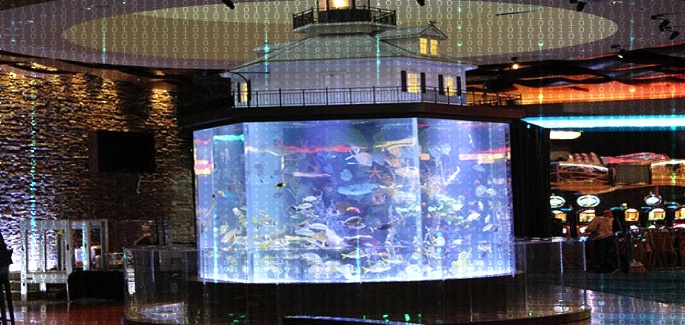
\includegraphics[width=\linewidth]{figures/casino.jpg}
        \caption*{\vspace{-0.5cm}\tiny\url{https://hackread.com/hackers-casinos-fish-tank-smart-thermometer-hack/}}
      \end{figure}

      \vspace{0.cm}
      \animategraphics[autoplay,loop,width=\linewidth]{1}{figures/cyberdefense_mas_frames/frame}{0}{8}

    \end{column}

  \end{columns}

\end{frame}


\begin{frame}{Introduction}{Research Problem}

  \begin{columns}

    \begin{column}{0.4\textwidth}
      \centering

      \begin{alertvarblock}[6cm]{General Research Question}
        Which \textbf{organizational mechanisms} in a cyber-defense MAS can \textbf{optimize its operation} while accounting for its \textbf{constraints}?
      \end{alertvarblock}

      \vspace{1em}

      \begin{itemize}
        \item \textbf{Search for an appropriate organization}
              \begin{itemize}
                \item Environmental constraints
                \item Design requirements
              \end{itemize}

              \vspace{1em}

        \item \textbf{Evaluation criteria:}
              \begin{itemize}
                \item[(C1)] Autonomy
                \item [(C2)] Performance
                \item [(C3)] Adaptation
                \item [(C4)] Control
                \item [(C5)] Explainability
              \end{itemize}
      \end{itemize}

    \end{column}

    \begin{column}{0.6\textwidth}
      % \resizebox{0.5\textwidth}{!}{
      \centering
      % 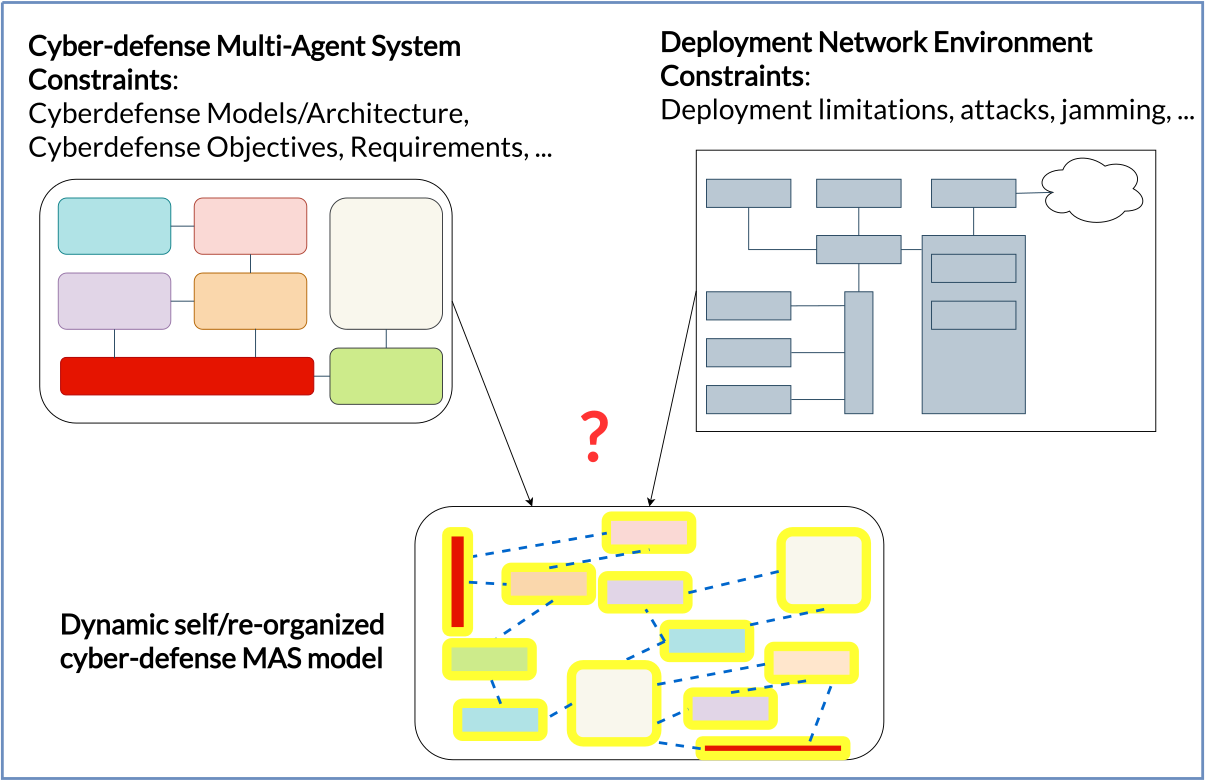
\includegraphics[width=0.95\linewidth]{figures/general_problem_illustration.png}
      \vspace{0.1cm}
      \resizebox{1\linewidth}{!}{\input{figures/problem_illustration}}
      % }
    \end{column}

  \end{columns}

\end{frame}

\begin{frame}{Outline}
  \tableofcontents
\end{frame}

\section{State of the Art}


\begin{frame}{}
  \tableofcontents[currentsection]
\end{frame}


\begin{frame}{State of the Art}{Overview of Related Work}

  \vspace{-0.5cm}

  \begin{adjustbox}{width=\linewidth, center}
    \setlength{\tabcolsep}{6pt}
\renewcommand{\arraystretch}{-1}

\begin{tabular}{
  >{\centering\arraybackslash}p{3.5cm}|   % nouvelle colonne regroupement
  p{7cm}
  >{\centering\arraybackslash}p{3cm}
  >{\centering\arraybackslash}p{1.8cm}
  >{\centering\arraybackslash}p{1.8cm}
  >{\centering\arraybackslash}p{1.8cm}
  >{\centering\arraybackslash}p{1.8cm}
  }
  \rowcolor{black!10}
  \textbf{AI family trend} & \textbf{Work category}                                            & \textbf{C1 Autonomy}               & \textbf{C2 Perf.}                   & \textbf{C3 Adapt.}                  & \textbf{C4 Control}                 & \textbf{C5 Explain.} \\
  \hline

  % ------------------------- SYMBOLIQUE -------------------------
  \multirow{3}{*}[-0.35cm]{\vspace{0.9cm}\textbf{$\sim$ \textit{Symbolic}}}
                           & {\vspace{0.25cm}\textbf{Expert systems $\sim$ cyber-defense MAS}}

    {\tiny \begin{spacing}{0.8}
               \textbf{hierarchies \& swarms}~\parencite{holloway2009self,lamont2009military,holloway2019self}, \textbf{evolutionary methods}~\parencite{akandwanaho2018generic,carvalho2011evolutionary}, \textbf{reactive architectures}~\parencite{de2017distributed}, \textbf{bio-inspired methods}~\parencite{haack2011ant}, \textbf{cyber-physical frameworks}~\parencite{demir2021adaptive}, \textbf{CIDS}~\parencite{vasilomanolakis2015taxonomy}
             \end{spacing}}






                           & {\vspace{0.65cm}\xmark~--~$\sim$}                                 & {\vspace{0.65cm} $\sim$ }          & {\vspace{0.65cm} $\sim$ }           & {\vspace{0.65cm} \cmark }           & {\vspace{0.65cm} \cmark }                                  \\

                           & \textbf{Environment modeling}
  {\tiny \begin{spacing}{0.8}
             \textbf{formal models (POMDP, Dec-POMDP, POSG)}~\parencite{Oliehoek2016, Beynier2013}, \textbf{game theory}~\parencite{MPanfili2018,AAttiah2018,CXiaolin2008}, \textbf{attack graphs}~\parencite{CPhilips1998}, \textbf{attack-defense trees}~\parencite{BKordy2010}, \textbf{Petri nets}~\parencite{SYamaguchi2020}
           \end{spacing}}


                           & {\vspace{0.2cm} \xmark }                                          & {\vspace{0.2cm} $\sim$    }        & {\vspace{0.2cm} $\sim$ }            & {\vspace{0.2cm} \cmark }            & {\vspace{0.2cm} \cmark }                                   \\

                           & \textbf{MAS design frameworks}
  {\tiny \begin{spacing}{0.8}
             \textbf{network simulation}~\parencite{Standen2021, janisch2023nasimemu}, \textbf{training frameworks}~\parencite{hammar_stadler_noms_22, CROND}, \textbf{experimental platforms}~\parencite{Niculae2018, cyberbattlesim}
           \end{spacing}}
                           & {\vspace{0.12cm}\cmark }                                          & {\vspace{0.12cm} \cmark  }         & {\vspace{0.12cm} $\sim$~--~\cmark } & {\vspace{0.12cm} \xmark }           & {\vspace{0.12cm} \xmark~--~$\sim$ }                        \\

  \vspace{-4.35cm}

  \multirow{1}{*}{
    \begin{tikzpicture}
      \draw[<->, thick] (0,1)--(0,8);
      \vspace{1cm}
    \end{tikzpicture}
  }



  % ---------------------- CONNEXIONNISTE ------------------------
  \multirow{3}{*}{\vspace{-13.8cm}\textbf{$\sim$ \textit{Connectionist}}}
  \vspace{-0.35cm}
                           & \textbf{Maintaining simulation/real-world consistency}

  {\tiny \begin{spacing}{0.8}
             \textbf{Robust RL}~\parencite{pinto2017robust}, \textbf{Sim2Real}~\parencite{tobin2017domain,ganin2016domain}, \textbf{dynamic calibration}~\parencite{deisenroth2011pilco}
           \end{spacing}}

                           & {\vspace{-0.12cm}$\sim$~--~\cmark }                               & {\vspace{-0.12cm}n/a }             & {\vspace{-0.12cm} \cmark }          & {\vspace{-0.12cm} $\sim$ }          & {\vspace{-0.12cm} $\sim$ }                                 \\

                           & \textbf{MARL \& organizational constraints}

  {\tiny \begin{spacing}{0.8}
             \textbf{CPO}~\parencite{achiam2017constrained}, \textbf{Deep Constrained Q-Learning}~\parencite{kalweit2020deep}, \textbf{Safe RL}~\parencite{garcia2015comprehensive}, \textbf{Deep TAMER}~\parencite{warnell2018deep}, \textbf{reward shaping}~\parencite{ng1999policy}, \textbf{shielding}~\parencite{amodei2016concrete}
           \end{spacing}}

                           & {\vspace{0.06cm}\xmark~--~$\sim$ }                                & {\vspace{0.06cm}$\sim$~--~\cmark } & {\vspace{0.06cm} $\sim$ }           & {\vspace{0.06cm} \cmark }           & {\vspace{0.06cm} $\sim$~--~\cmark }                        \\

                           & \textbf{Emergent organizational extraction}
  {\tiny \begin{spacing}{0.8}
             \textbf{tree extraction}~\parencite{milani2022maviper,zhang2024advancing}, \textbf{value decompositions}~\parencite{Sunehag2018,Tabish2018}, \textbf{Shapley attributions}~\parencite{heuillet2021collective}, \textbf{emergent role inference}~\parencite{Wang2020}
           \end{spacing}}

                           & {\vspace{0.06cm} \xmark~--~$\sim$ }                               & {\vspace{0.06cm} $\sim$  }         & {\vspace{0.06cm} $\sim$ }           & {\vspace{0.06cm} \xmark~--~$\sim$ } & {\vspace{0.06cm} \cmark }                                  \\[0.001cm]
  \hline
\end{tabular}

  \end{adjustbox}

  \vspace{0.5cm}

  $\Longrightarrow$ \textbf{Approaches: \textquote{Symbolic AI} // \textquote{Connectionist AI}} \\ \ \\

  \vspace{-0.cm}

  \noindent {\tiny \begin{spacing}{0.8}
      \textit{Soulé, J., Jamont, J.-P., Occello, M., Traonouez L.-M., Théron, P. (2023). On the Organization of a Cyber-Defense Multi-Agent System. In the Proceedings of the French Conference on Research and Education in Information Systems Security (RESSI 2023). France.}
    \end{spacing}}

  \vspace{-1.5cm}

\end{frame}


\begin{frame}{State of the Art}{Recommendations: Problem Decomposition \& Hypotheses}
  \centering
  \setlength{\tabcolsep}{8pt}
  \renewcommand{\arraystretch}{1.5}
  \setlength{\extrarowheight}{2pt}

  \resizebox{\linewidth}{!}{
    \begin{tabular}{lp{6.5cm}p{5cm}}
      \hline
      \textbf{Sub-problem}     & \textbf{Hypothesis}                                                                                     & \textbf{Criteria C1--C5}      \\
      \hline
      \textbf{Modeling -- MOD} & \textbf{H-MOD}: Obtaining a realistic simulated environment (manually or through learning).             & C1 Autonomy, C3 Adaptation    \\

      \textbf{Training -- TRN} & \textbf{H-TRN}: Integrating organizational constraints into MARL to obtain safe and compliant policies. & C2 Performance, C4 Control    \\

      \textbf{Analysis -- ANL} & \textbf{H-ANL}: Automatically inferring organizational roles and goals from agent trajectories.         & C4 Control, C5 Explainability \\

      \textbf{Transfer -- TRF} & \textbf{H-TRF}: Simulation-to-real coupling (digital twin) enabling safe and adaptive transfer.         & C1 Autonomy, C3 Adaptation    \\
    \end{tabular}}
\end{frame}



\section{Method}

\begin{frame}{}

  \vspace{1cm}

  \begin{columns}[T]
    \begin{column}{0.5\textwidth}
      \tableofcontents[currentsection]

      \vspace{0.5cm}

      \begin{itemize}
        \item[(1)] Model the environment manually / automatically;
        \item[(2)] Train agents with MARL + constraints;
      \end{itemize}

      \vspace{-2.5cm}

    \end{column}
    \hspace{-1cm}
    \begin{column}{0.5\textwidth}
      \centering
      \vspace{-0.3cm}

      \begin{figure}[h]
        \centering
        \begin{tikzpicture}
          % Image complète (non coupée)
          \node[anchor=south west,inner sep=0] (img)
          {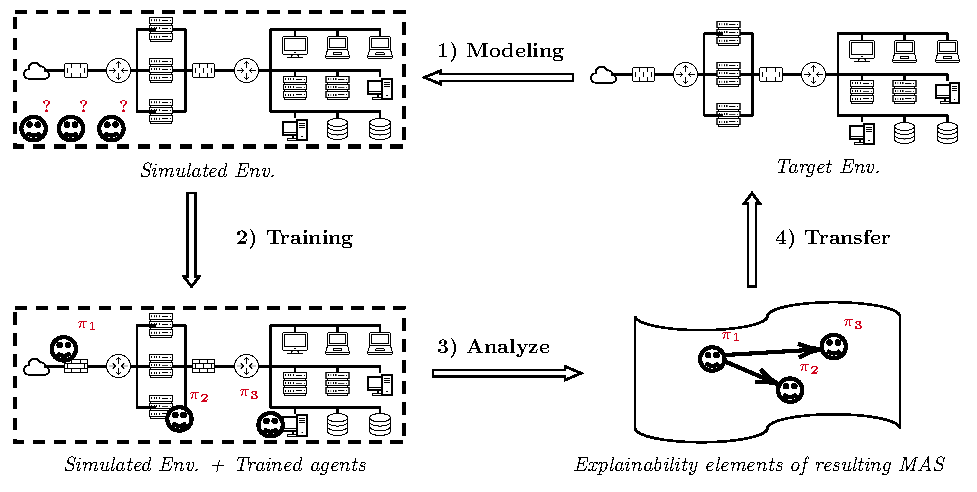
\includegraphics[width=1.1\linewidth]{figures/en_cycle.pdf}};

        \end{tikzpicture}
      \end{figure}

      \begin{itemize}
        \item[(3)] Analyze emergent roles and goals;
        \item[(4)] Transfer policies and environment dynamics from simulation to reality.
      \end{itemize}

      \vspace{-1cm}

    \end{column}
  \end{columns}

  \vspace{1.85cm}

  \noindent {\tiny \begin{spacing}{0.8}
      \textit{Soulé, J., Jamont, J.-P., Occello, M., Traonouez L.-M., Théron, P. (2025). \textquote{Assisting Multi-Agent System Design with $\mathcal{M}OISE^+$ and MARL : The MAMAD Method}. In : Journal of Autonomous Agents and Multi-Agent Systems (JAAMAS) (2025). Under revision.}
    \end{spacing}}

\end{frame}

% \subsection{Aperçu général}

% \begin{frame}{Méthode}{Aperçu général}

%   \begin{columns}[c]

%     \hspace{-1.5cm}

%     \begin{column}{0.5\textwidth}
%       \begin{enumerate}
%         \item Modéliser l'environnement manuellement / automatiquement ;
%         \item Entraînement des agents à l'aide de MARL + Contraintes ;
%         \item Analyse pour rôles et objectifs émergents des agents ;
%         \item Transferer politiques en simulation vers réel + maitenir fidelité environnement simulé.
%       \end{enumerate}

%     \end{column}

%     \hspace{-1.5cm}

%     \begin{column}{0.5\textwidth}
%       \begin{figure}[h!]
%         \centering
%         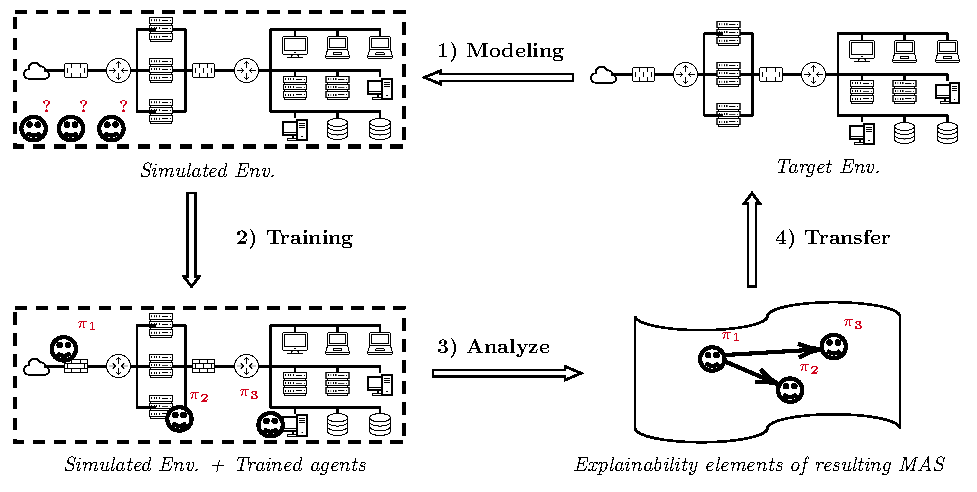
\includegraphics[width=1.2\linewidth]{figures/en_cycle.pdf}
%         \label{fig:cycle}
%       \end{figure}
%     \end{column}
%   \end{columns}

%   \noindent {\tiny \begin{spacing}{0.8}
%       \textit{Soulé, J., Jamont, J.-P., Occello, M., Traonouez L.-M., Théron, P. (2025). \textquote{Assisting Multi-Agent System Design with $\mathcal{M}OISE^+$ and MARL : The MAMAD Method}. In : Journal of Autonomous Agents and Multi-Agent Systems (JAAMAS) (2025). Under revision.}
%     \end{spacing}}

% \end{frame}



\subsection{Modeling}

\begin{frame}{}
  \begin{columns}[T]
    \begin{column}{0.5\textwidth}
      \tableofcontents[currentsubsection]
    \end{column}
    \begin{column}{0.5\textwidth}
      \centering
      \vspace{0.5cm}

      \begin{figure}[h]
        \centering
        \begin{tikzpicture}
          % Image complète (non coupée)
          \node[anchor=south west,inner sep=0] (img)
          {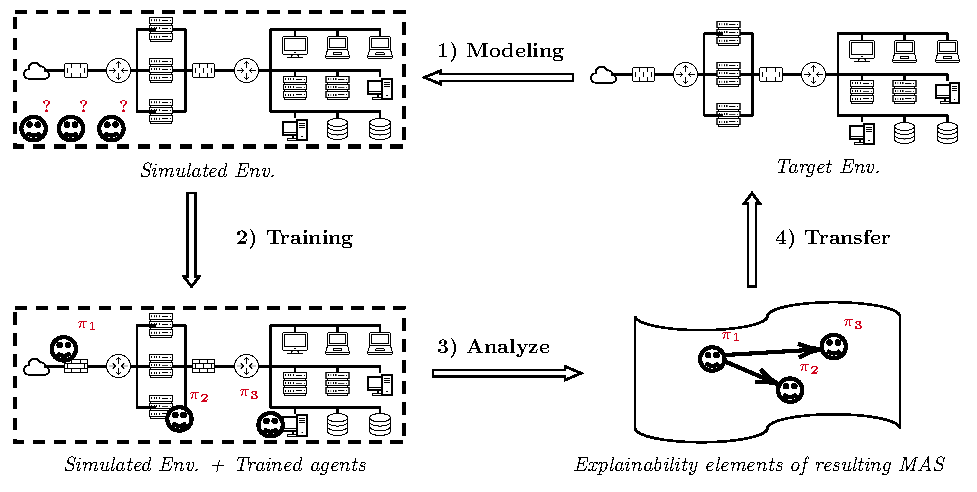
\includegraphics[width=\linewidth]{figures/en_cycle.pdf}};

          % % Masque gris semi-transparent sur toute l'image
          \fill[white,opacity=0.6] (0,0) rectangle (\linewidth,2.15);

        \end{tikzpicture}
      \end{figure}


    \end{column}
  \end{columns}
\end{frame}

\begin{frame}{Simulation-Based Modeling}{Setting}

  \textbf{A networked environment}
  \begin{itemize}
    \item Properties: open, dynamic/static, deterministic, accessible/inaccessible\dots
          \phantom{XXXXXXXXXXXXXXXXXXXXXXXXXXXXXXXXXXXXXXXXXXXXXXXXX}
  \end{itemize}

  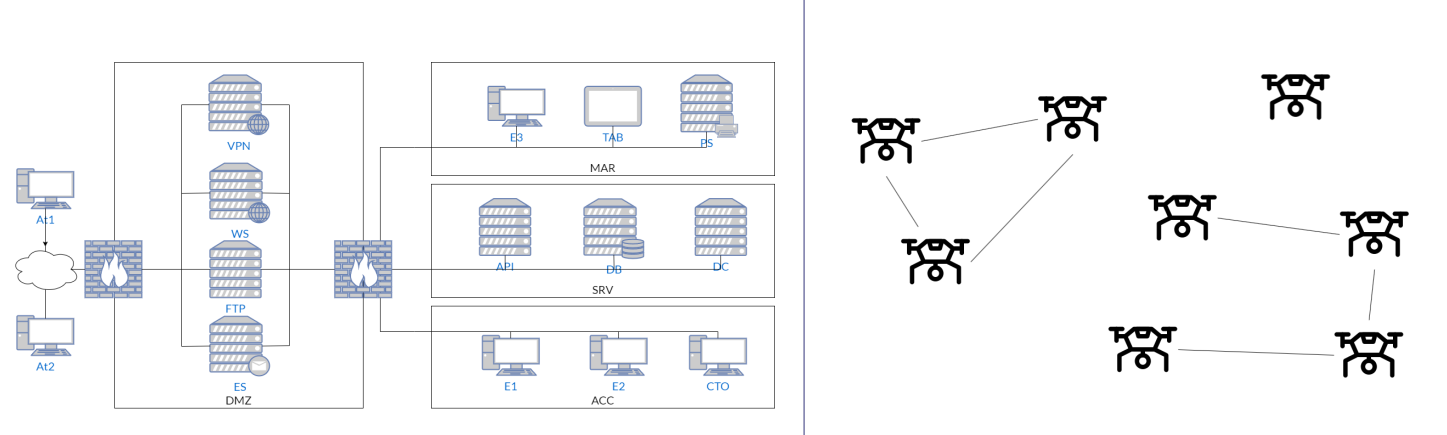
\includegraphics[width=\linewidth, trim=0cm 0cm 0cm 0.1cm, clip]{figures/0.png}

\end{frame}

\begin{frame}{Simulation-Based Modeling}{Setting}

  \textbf{With a Green Team}
  \begin{itemize}
    \item Nominal users: sessions, requests, port scans, data transmission
          \phantom{XXXXXXXXXXXXXXXXXXXXXXXXXXXXXXXXXXXXXXXXXXXXXXXXXXXXXXXXXXXXXXXX}
  \end{itemize}

  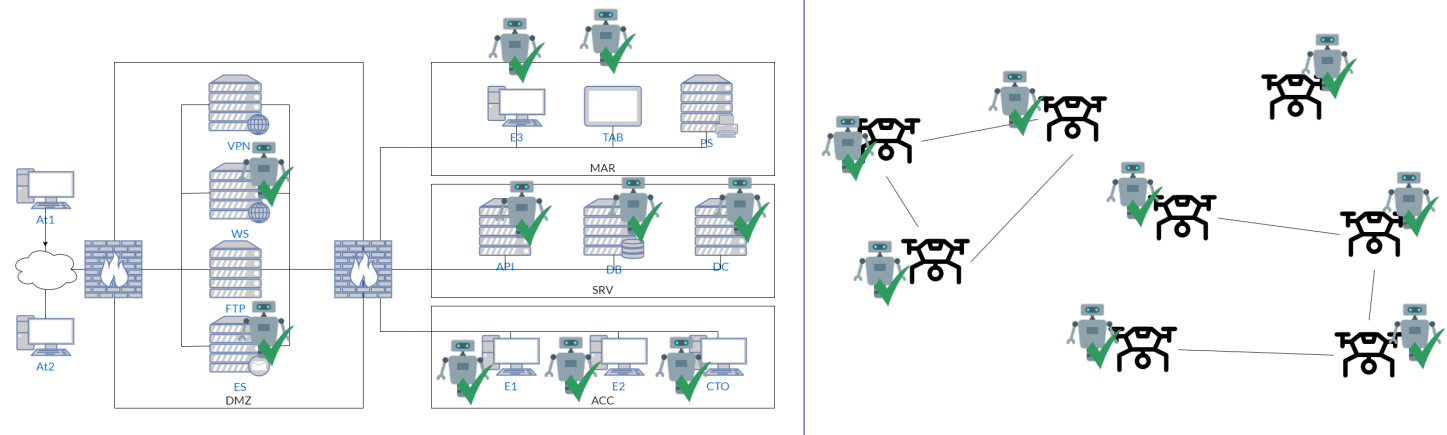
\includegraphics[width=\linewidth, trim=0cm 0cm 0cm 0.1cm, clip]{figures/1.png}
\end{frame}

\begin{frame}{Simulation-Based Modeling}{Setting}

  \textbf{With a Red Team}
  \begin{itemize}
    \item Cyber attackers: node/service discovery, vulnerability exploitation, privilege escalation, lateral movement, impact\dots
  \end{itemize}

  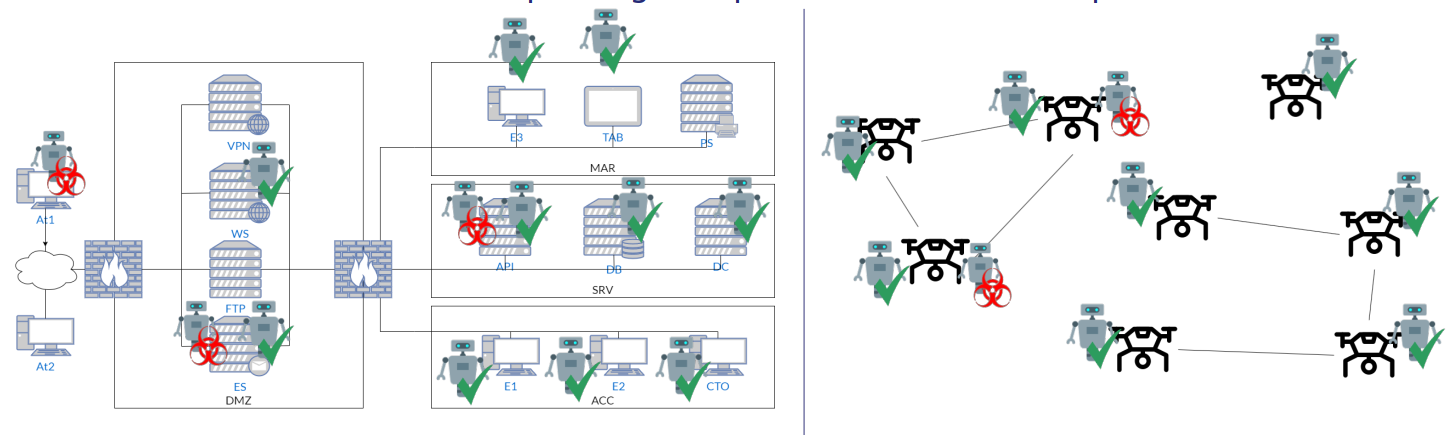
\includegraphics[width=\linewidth, trim=0cm 0cm 0cm 0.1cm, clip]{figures/2.png}
\end{frame}

\begin{frame}{Simulation-Based Modeling}{Setting}

  \textbf{With a Blue Team}
  \begin{itemize}
    \item Cyber defenders: threat analysis, access control, terminating suspicious processes, deploying honeypots, re-imaging a node\dots
  \end{itemize}

  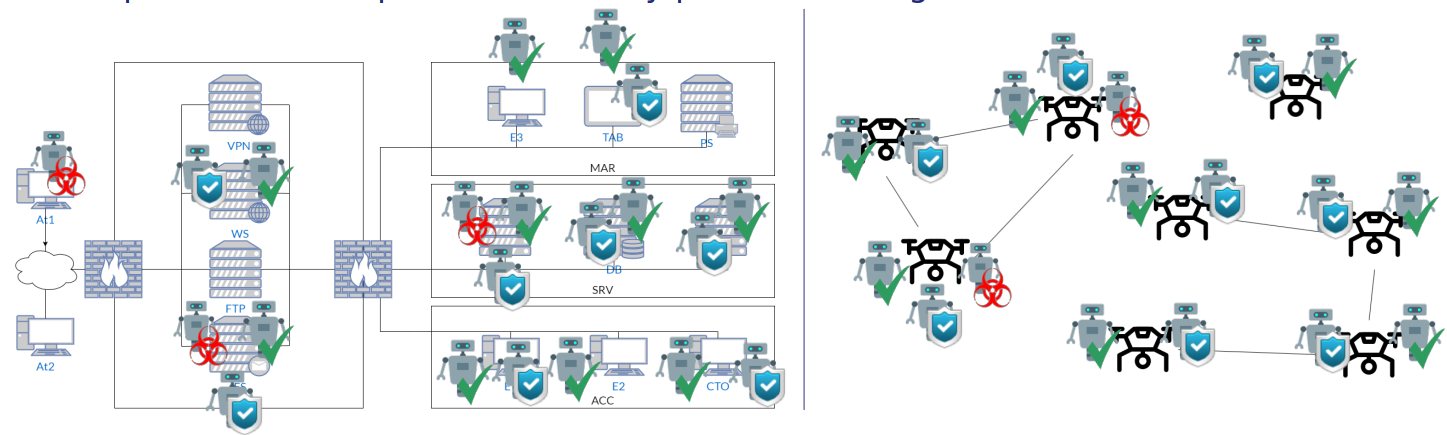
\includegraphics[width=\linewidth, trim=0cm 0cm 0cm 0.1cm, clip]{figures/3.png}
\end{frame}

\begin{frame}{Simulation-Based Modeling}{Markovian Model}

  \begin{columns}[c]

    \hspace{-1cm}

    \begin{column}{0.4\textwidth}

      \begin{itemize}
        \item Markovian model (Dec-POMDP) \\ \parencite{Oliehoek2016}
              \begin{itemize}
                \item Collective decision-making
                \item Modeling action / observation uncertainty
                \item \textbf{$T$: state transition function}
              \end{itemize}

        \item[\phantom{X}] \phantom{Manual modeling of $T$}
              \begin{itemize}
                \item[\phantom{X}] \phantom{CybORG}
              \end{itemize}
        \item[\phantom{X}] \phantom{Automated modeling of $T$}
              \begin{enumerate}
                \item[\phantom{X}] \phantom{Collecting real traces}
                \item[\phantom{X}] \phantom{Training with an RNN (LSTM)}
              \end{enumerate}
      \end{itemize}

    \end{column}

    \begin{column}{0.6\textwidth}
      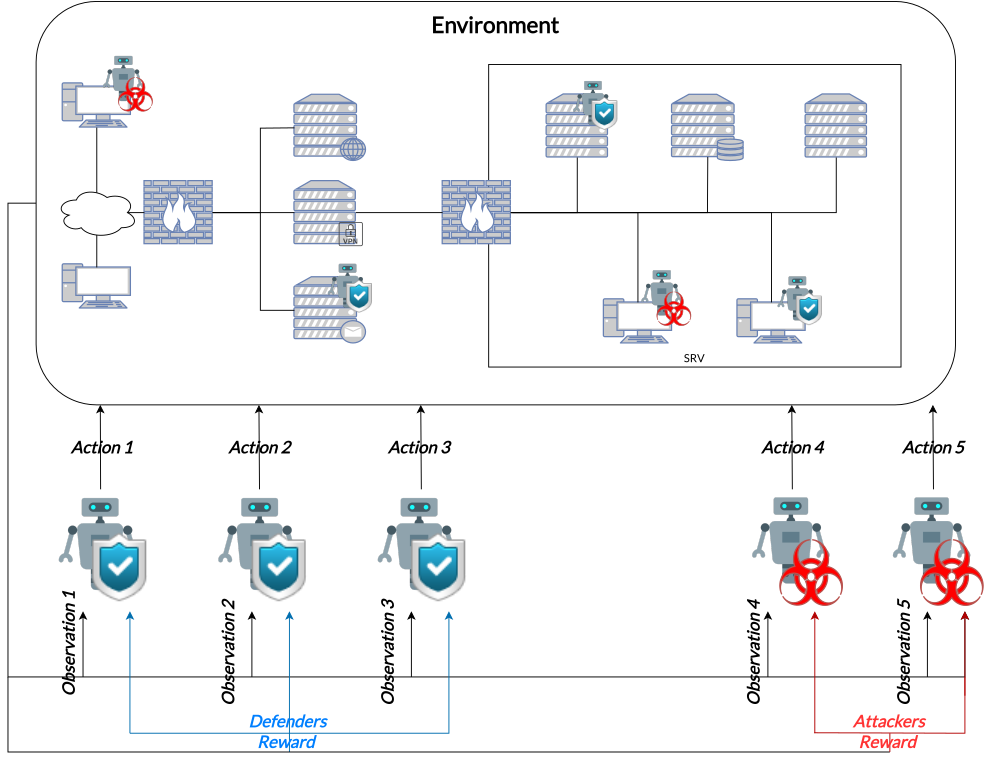
\includegraphics[width=\linewidth]{figures/marl_framework.png}
    \end{column}
  \end{columns}

  \vspace{0.2cm}

  {\centering \tiny \begin{spacing}{0.8}
      \textit{Soulé, J., Jamont, J.-P., Occello, M., Traonouez L.-M., Théron, P. Towards a Multi-Agent Simulation of Cyber-attackers and Cyber-defenders Battles. IEEE SMC 2023.}
    \end{spacing}}

\end{frame}


\begin{frame}{Simulation-Based Modeling}{Markovian Model}

  \begin{columns}[c]

    \hspace{-1.0cm}

    \begin{column}{0.4\textwidth}

      \begin{itemize}
        \item Markovian model (Dec-POMDP) \\ \parencite{Oliehoek2016}
              \begin{itemize}
                \item Collective decision-making
                \item Modeling action / observation uncertainty
                \item \textbf{$T$: state transition function}
              \end{itemize}

              \vspace{0.2cm}

        \item Manual modeling of $T$
              \begin{itemize}
                \item Simulators / emulators: CybORG \allowbreak \parencite{Maxwell2021}
              \end{itemize}
        \item[\phantom{X}] \phantom{Automated modeling of $T$}
              \begin{enumerate}
                \item[\phantom{X}] \phantom{Collecting real traces}
                \item[\phantom{X}] \phantom{Training with an RNN (LSTM)}
              \end{enumerate}
      \end{itemize}

    \end{column}

    \begin{column}{0.6\textwidth}
      \begin{table}[h!]
    \centering
    \renewcommand{\arraystretch}{2}
    \tiny
    \resizebox{\textwidth}{!}{%
        \begin{tabular}{
            p{1.5cm}
            >{\centering\arraybackslash}p{2.25cm}
            >{\centering\arraybackslash}p{2.25cm}
            >{\centering\arraybackslash}p{2.25cm}
            >{\centering\arraybackslash}p{2.25cm}
            >{\centering\arraybackslash}p{2.25cm}}
            \toprule
            \textbf{Framework}       & \textbf{C1 Autonomy}                                   & \textbf{C2 Performance}                       & \textbf{C3 Adaptation}                                  & \textbf{C4 Control}                    & \textbf{C5 Explainability}               \\
            \midrule
            \textbf{CybORG}          & Partial (simulated agents, but human guidance required) & Strong (broad range of scenarios)            & Partial (adaptive attackers, limited defenders)         & Weak (few explicit constraints)        & Weak (trajectories remain hard to interpret) \\
            \textbf{NASimEmu}        & Partial                                                & Strong (simulation granularity)               & Partial (topology variants)                             & Weak                                   & Weak                                     \\
            \textbf{CSLE}            & Partial                                                & Strong (multi-agent \textbf{RL})              & Partial (adaptation limited to fixed environments)      & Partial (parameter-based control)      & Partial (policy visualization)           \\
            \textbf{AutoPentest-DRL} & Weak (attacker-centered)                               & Strong (efficient scenario generation)        & Weak (limited defender-side adaptation)                 & Weak                                   & Weak                                     \\
            \textbf{EmuLab}          & Weak (limited agent autonomy)                          & Strong (network realism)                      & Weak (manual adaptation)                                & Weak                                   & Weak                                     \\
            \textbf{CLAP}            & Partial                                                & Strong (multiple objectives)                  & Partial (co-evolution of strategies)                    & Weak                                   & Weak                                     \\
            \textbf{CyberBattleSim}  & Partial                                                & Strong (\textbf{RL} policy comparison)        & Partial (diverse vulnerability graphs)                  & Weak                                   & Weak                                     \\
            \textbf{CANDLES}         & Partial                                                & Strong (co-evolution of defense/attack agents) & Strong (evolution-driven adaptation)                   & Weak                                   & Weak                                     \\
            \textbf{PenGym}          & Weak                                                   & Partial (focused on pentesting)               & Weak                                                    & Weak                                   & Weak                                     \\
            \textbf{ASAP}            & Weak                                                   & Partial (automated analysis)                  & Weak                                                    & Weak                                   & Weak                                     \\
            \bottomrule
        \end{tabular}
    }% fin resizebox
\end{table}

      {\tiny \begin{spacing}{0.8}
          \tiny Indicative scale: \textit{Weak} = not addressed or only marginally; \textit{Partial} = partially covered, depending on scenarios; \textit{Strong} = explicit and generalizable support.
        \end{spacing}}

    \end{column}
  \end{columns}

  \vspace{1.2cm}

  {\centering \tiny \begin{spacing}{0.8}
      \textit{Soulé, J., Jamont, J.-P., Occello, M., Traonouez L.-M., Théron, P. Towards a Multi-Agent Simulation of Cyber-attackers and Cyber-defenders Battles. IEEE SMC 2023.}
    \end{spacing}}

\end{frame}



\begin{frame}{Simulation-Based Modeling}{Markovian Model}

  \vspace{1cm}

  \begin{columns}[c]

    \hspace{-0.6cm}

    \begin{column}{0.5\textwidth}

      \vspace{-0.5cm}
      \begin{itemize}
        \item Markovian model (Dec-POMDP) \\ \parencite{Oliehoek2016}
              \begin{itemize}
                \item \textbf{$T$: state transition function $\rightarrow \sensinterdit$}
                      \begin{itemize}
                        \item[$\Longrightarrow$] $\mathcal{T}$ captures $O + T$: transition + observation
                      \end{itemize}
              \end{itemize}

              \vspace{0.2cm}

        \item Automated modeling of $\mathcal{T}$
              \begin{itemize}
                \item Trajectory dataset
                \item \textit{World Models}~\parencite{Ha2018}
                \item Observation Prediction Model
                      \begin{itemize}
                        \item Predicts the next observation
                      \end{itemize}
              \end{itemize}
      \end{itemize}

    \end{column}

    \hspace{-0.8cm}

    \begin{column}{0.6\textwidth}

      \vspace{0cm}

      \centering

      \resizebox{0.8\linewidth}{!}{\input{figures/single_agent_world_model.tex}}

      \vspace{0.3cm}

    \end{column}
  \end{columns}

  \vspace{1.4cm}

  \noindent {\tiny \begin{spacing}{0.8}
      \textit{Soulé, J., Jamont, J.-P., Occello, M., Traonouez L.-M., Théron, P. (2025). \textquote{Assisting Multi-Agent System Design with $\mathcal{M}OISE^+$ and MARL : The MAMAD Method}. In : Journal of Autonomous Agents and Multi-Agent Systems (JAAMAS) (2025). Under revision.}
    \end{spacing}}

\end{frame}




\begin{frame}{Simulation-Based Modeling}{Markovian Model}

  \vspace{1cm}

  \begin{columns}[c]

    \hspace{-0.6cm}

    \begin{column}{0.5\textwidth}

      \vspace{-0.5cm}
      \begin{itemize}
        \item Markovian model (Dec-POMDP) \\ \parencite{Oliehoek2016}
              \begin{itemize}
                \item \textbf{$T$: state transition function $\rightarrow \sensinterdit$}
                      \begin{itemize}
                        \item[$\Longrightarrow$] $\mathcal{T}^j$ captures $O + T$: transition + observation
                      \end{itemize}
              \end{itemize}

              \vspace{0.2cm}

        \item Automated modeling of \textit{multi-agent} $\mathcal{T}^j$
              \begin{itemize}
                \item Joint trajectory dataset
                \item Based on \textit{World~Models} \\ \parencite{Ha2018}
                \item Joint-Observation Prediction Model
                      \begin{itemize}
                        \item Predicts the next joint observation
                      \end{itemize}
              \end{itemize}
      \end{itemize}

    \end{column}

    \hspace{-0.8cm}

    \begin{column}{0.6\textwidth}

      \vspace{-1cm}

      \centering

      \resizebox{\linewidth}{!}{\input{figures/jopm_synthesis.tex}}

    \end{column}
  \end{columns}

  \vspace{1.4cm}

  \noindent {\tiny \begin{spacing}{0.8}
      \textit{Soulé, J., Jamont, J.-P., Occello, M., Traonouez L.-M., Théron, P. (2025). \textquote{Assisting Multi-Agent System Design with $\mathcal{M}OISE^+$ and MARL : The MAMAD Method}. In : Journal of Autonomous Agents and Multi-Agent Systems (JAAMAS) (2025). Under revision.}
    \end{spacing}}

\end{frame}



\subsection{Training}

\begin{frame}{}
  \begin{columns}[T]
    \begin{column}{0.5\textwidth}
      \tableofcontents[currentsubsection]
    \end{column}
    \begin{column}{0.5\textwidth}
      \centering
      \vspace{0.5cm}

      \begin{figure}[h]
        \centering
        \begin{tikzpicture}
          % Image complète (non coupée)
          \node[anchor=south west,inner sep=0] (img)
          {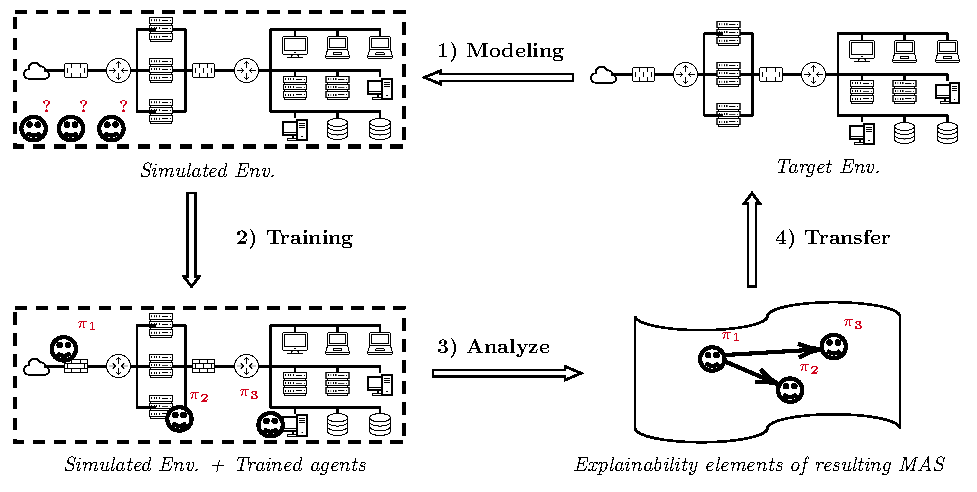
\includegraphics[width=\linewidth]{figures/en_cycle.pdf}};

          % % Masque gris semi-transparent sur toute l'image
          \fill[white,opacity=0.6] (0.425\linewidth,0) rectangle (\linewidth,3.4);

        \end{tikzpicture}
      \end{figure}

    \end{column}
  \end{columns}
\end{frame}


\begin{frame}{Training}{Standard MARL}

  \begin{itemize}
    \item Select the best actions to maximize cumulative reward
  \end{itemize}

  \begin{center}
    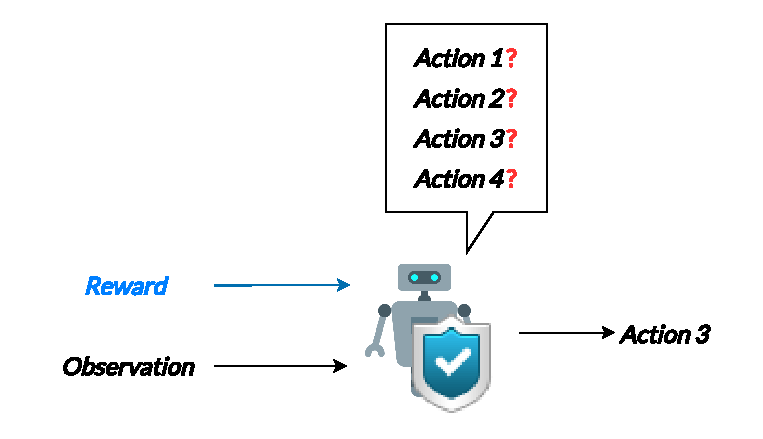
\includegraphics[width=0.5\linewidth]{figures/vanilla_marl.pdf}
  \end{center}

  % \vfill

  % {\tiny \begin{spacing}{0.8}
  %     \textit{Soulé, J., Jamont, J.-P., Occello, M., Traonouez L.-M., Théron, P. An Organizationally-Oriented Approach to Enhancing Explainability and Control in Multi-Agent Reinforcement Learning. Proceedings of the 24th International Conference on Autonomous Agents and Multiagent Systems (AAMAS 2025), Detroit, Michigan, USA, 2025.}
  %   \end{spacing}}

\end{frame}

\begin{frame}{Training}{Guided / Constrained Learning}

  \textbf{MARL + organization}
  \begin{itemize}
    \item Role: enforce / forbid actions $\rightarrow$ safety guarantee
  \end{itemize}

  \begin{center}
    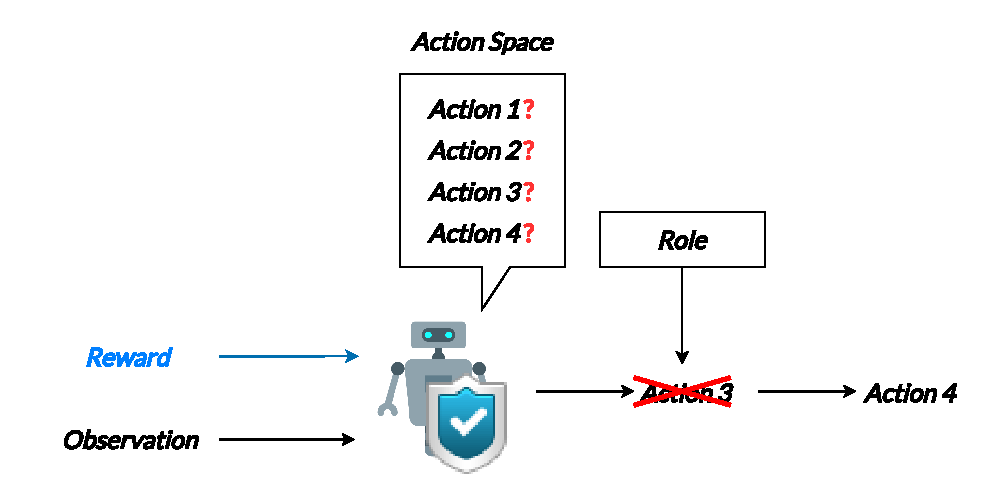
\includegraphics[width=0.5\linewidth]{figures/role_marl.pdf}
  \end{center}

  % \vfill

  % {\tiny \begin{spacing}{0.8}
  %     \textit{Soulé, J., Jamont, J.-P., Occello, M., Traonouez L.-M., Théron, P. An Organizationally-Oriented Approach to Enhancing Explainability and Control in Multi-Agent Reinforcement Learning. Proceedings of the 24th International Conference on Autonomous Agents and Multiagent Systems (AAMAS 2025), Detroit, Michigan, USA, 2025.}
  %   \end{spacing}}

\end{frame}

\begin{frame}{Training}{Guided / Constrained Learning}

  \textbf{MARL + organization}
  \begin{itemize}
    \item Goal: encourage the achievement of an intermediate objective
  \end{itemize}

  \begin{center}
    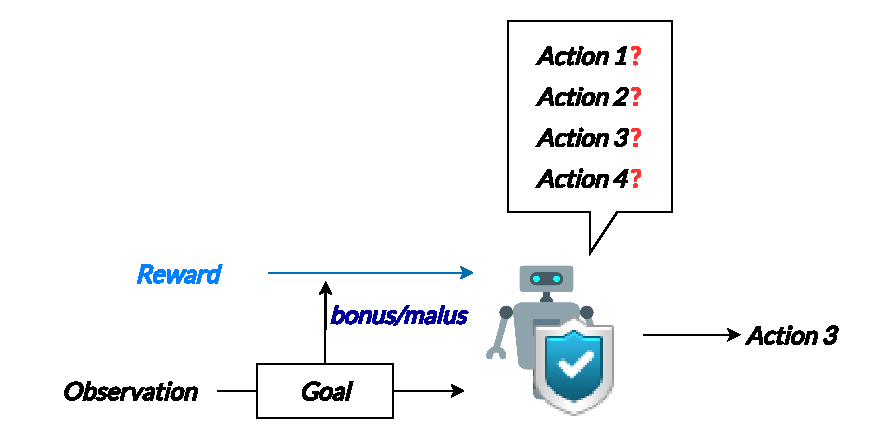
\includegraphics[width=0.5\linewidth]{figures/goal_marl.pdf}
  \end{center}

  % \vfill

  % {\tiny \begin{spacing}{0.8}
  %     \textit{Soulé, J., Jamont, J.-P., Occello, M., Traonouez L.-M., Théron, P. An Organizationally-Oriented Approach to Enhancing Explainability and Control in Multi-Agent Reinforcement Learning. Proceedings of the 24th International Conference on Autonomous Agents and Multiagent Systems (AAMAS 2025), Detroit, Michigan, USA, 2025.}
  %   \end{spacing}}

\end{frame}

\begin{frame}{Training}{The MOISE+MARL Framework}

  \begin{columns}[c] % c = vertically center content
    \begin{column}{0.5\textwidth}
      \begin{itemize}
        \item Combine Dec-POMDP with $\mathcal{M}OISE^+$.
        \item Agents $\rightarrow$ role and mission $\rightarrow$ goals.
        \item Constraint guides $\sim$ \textquote{role / goal implementation}:
              \begin{itemize}
                \item \textbf{Actions} via \textit{RoleActionGuides} (RAG)
                \item \textbf{Rewards} via \textit{RoleRewardGuides} and \textit{GoalRewardGuides}
              \end{itemize}
      \end{itemize}
    \end{column}
    \begin{column}{0.6\textwidth}
      \begin{figure}
        \centering

        \vspace{0.1cm}

        \resizebox{1\linewidth}{!}{
          \input{figures/mm_synthesis_single_column.tex}
        }


      \end{figure}
    \end{column}
  \end{columns}

  \vfill

  {\tiny \begin{spacing}{0.8}
      \textit{Soulé, J., Jamont, J.-P., Occello, M., Traonouez L.-M., Théron, P. An Organizationally-Oriented Approach to Enhancing Explainability and Control in Multi-Agent Reinforcement Learning. Proceedings of the 24th International Conference on Autonomous Agents and Multiagent Systems (AAMAS 2025), Detroit, Michigan, USA, 2025.}
    \end{spacing}}

\end{frame}



\subsection{Analysis}

\begin{frame}{}
  \begin{columns}[T]
    \begin{column}{0.5\textwidth}
      \tableofcontents[currentsubsection]
    \end{column}
    \begin{column}{0.5\textwidth}
      \centering
      \vspace{0.5cm}

      % \begin{figure}
      %   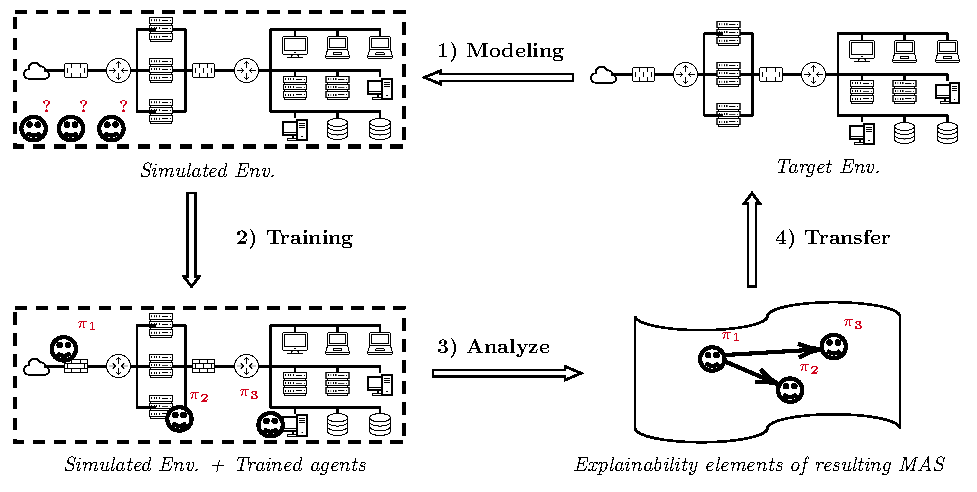
\includegraphics[trim={0cm 0cm 0cm 7.5cm},clip, width=\linewidth]{figures/en_cycle.pdf}
      % \end{figure}

      \begin{figure}[h]
        \centering
        \begin{tikzpicture}
          % Image complète (non coupée)
          \node[anchor=south west,inner sep=0] (img)
          {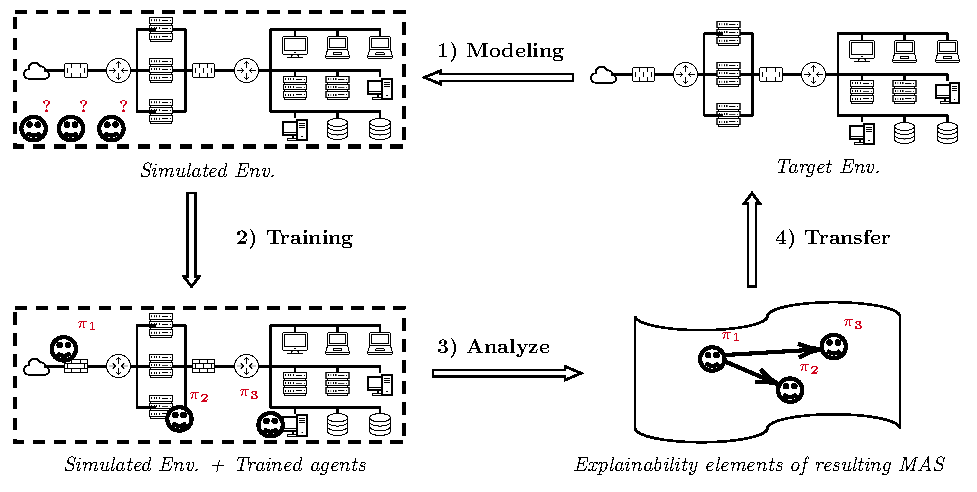
\includegraphics[width=\linewidth]{figures/en_cycle.pdf}};

          % % Masque gris semi-transparent sur toute l'image
          \fill[white,opacity=0.6] (0,3.4) rectangle (\linewidth,1.35);

        \end{tikzpicture}
      \end{figure}

    \end{column}
  \end{columns}
\end{frame}

\begin{frame}{Analysis}{Method Overview}

  \textbf{Trajectory-based Evaluation in MOISE+MARL (TEMM)}
  \begin{itemize}
    \item \textbf{Objective}: provide a post-hoc interpretation of agent behavior at the organizational level.
    \item \textbf{Hypothesis}: trajectories are \textquote{noisy} variants of a limited number of strategies.

  \end{itemize}

  \vspace{1em}
  \textbf{Underlying hypotheses:}
  \begin{itemize}
    \item \textbf{Roles} correspond to frequent \emph{(observation, action)} transition patterns in agent trajectories.
    \item \textbf{Goals} correspond to observations frequently received within agent trajectories.
  \end{itemize}

  \vspace{0.4cm}
  \begin{center}
    \begin{columns}[c]

      \begin{column}{0.4\textwidth}
        \centering
        \input{figures/abstract_obs_processed_viz.tex}
      \end{column}

      \begin{column}{0.1\textwidth}
      \end{column}

      \begin{column}{0.4\textwidth}
        \centering
        \input{figures/abstract_full_processed_viz.tex}
      \end{column}
    \end{columns}
  \end{center}

  \begin{tikzpicture}[remember picture, overlay]
    \node[anchor=north west, text=black]
    at ([xshift=5.8cm,yshift=-5cm]current page.north west) {\small
      \begin{minipage}{0.3\linewidth}
        {\small \hspace{0.8cm} \textit{\textbf{Operationalization\dots}}
          \begin{itemize}
            \item  \textit{Trajectories as vectors;}
            \item  \textit{Distances: Smith-Waterman, LCS, Euclidean\dots;}
            \item  \textit{Clustering + centroids \\ \ \ \ $\rightarrow$ roles / goals}
          \end{itemize}}
      \end{minipage}

    };
  \end{tikzpicture}

  \vspace{-0.5cm}

  {\tiny \begin{spacing}{0.8}
      \textit{Soulé, J., Jamont, J.-P., Occello, M., Traonouez L.-M., Théron, P. An Organizationally-Oriented Approach to Enhancing Explainability and Control in Multi-Agent Reinforcement Learning. Proceedings of the 24th International Conference on Autonomous Agents and Multiagent Systems (AAMAS 2025), Detroit, Michigan, USA, 2025.}
    \end{spacing}}

\end{frame}


\subsection{Transfer}

\begin{frame}{}
  \begin{columns}[T]
    \begin{column}{0.5\textwidth}
      \tableofcontents[currentsubsection]
    \end{column}
    \begin{column}{0.5\textwidth}
      \centering
      \vspace{0.5cm}

      \begin{figure}[h]
        \centering
        \begin{tikzpicture}
          % Image complète (non coupée)
          \node[anchor=south west,inner sep=0] (img)
          {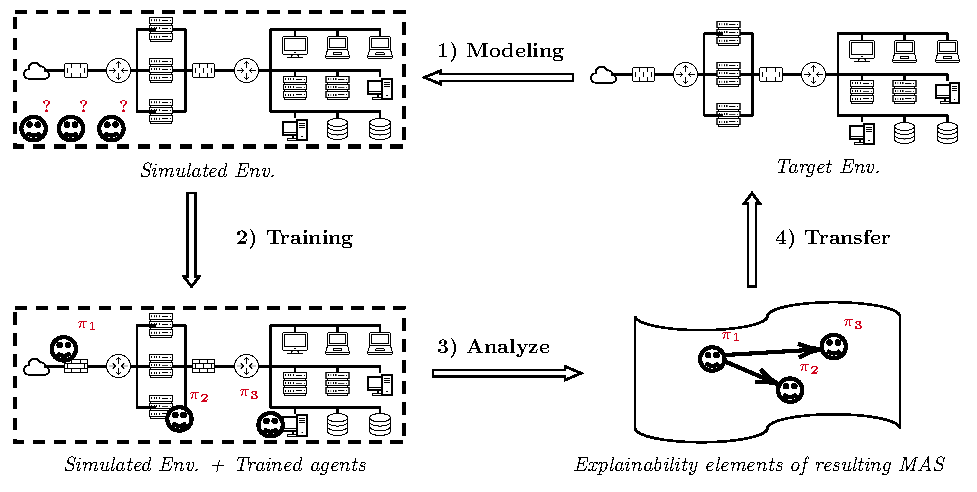
\includegraphics[width=\linewidth]{figures/en_cycle.pdf}};

          % % Masque gris semi-transparent sur toute l'image
          \fill[white,opacity=0.6] (0,0) rectangle (0.589\linewidth,3.7);

        \end{tikzpicture}
      \end{figure}

    \end{column}
  \end{columns}
\end{frame}

\begin{frame}{Transfer / Deployment}

  \begin{columns}
    \begin{column}{0.4\textwidth}
      \begin{itemize}
        \item Load and execute the policy remotely or directly; collect new transitions.
        \item Collect real trajectories in batches.
        \item Trigger model and policy updates.
      \end{itemize}
    \end{column}

    \begin{column}{0.6\textwidth}
      \vspace{-1cm}
      \begin{figure}
        \centering
        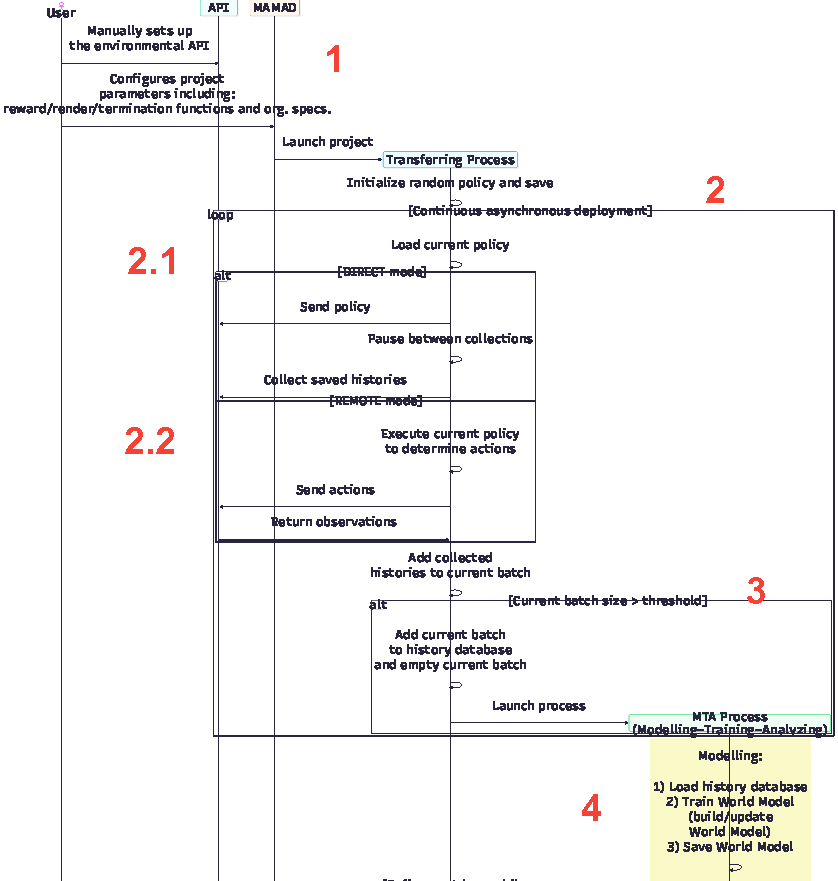
\includegraphics[width=0.95\textwidth]{figures/seq_diag_1.pdf}
      \end{figure}
    \end{column}
  \end{columns}

\end{frame}

\begin{frame}{Transfer / Deployment}

  \begin{columns}
    \begin{column}{0.4\textwidth}
      \begin{itemize}
        \item Update the simulation model from a trajectory dataset;
        \item Refinement cycles:
              \begin{itemize}
                \item (Re-)training policies
                \item Analyzing and manually adjusting the suggested organizational specifications
                \item Updating the policy
              \end{itemize}
      \end{itemize}
    \end{column}

    \begin{column}{0.6\textwidth}
      \begin{figure}
        \centering
        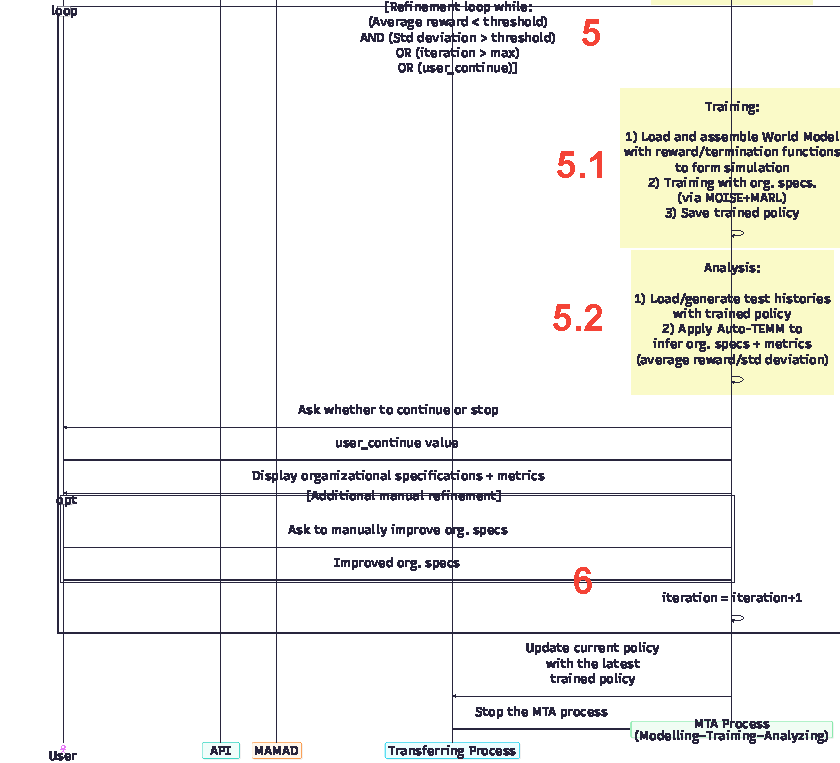
\includegraphics[width=0.95\textwidth]{figures/seq_diag_2.pdf}
      \end{figure}
    \end{column}
  \end{columns}

\end{frame}


\section{Implementation: CybMASDE}

\begin{frame}{}
  \tableofcontents[currentsection]
\end{frame}

\begin{frame}{Cyber(defense) Multi-Agent System Development Environment}

  \begin{columns}

    \hspace{-0.85cm}
    \begin{column}{0.4\textwidth}
      \begin{itemize}
        \item Desktop application (Electron):
              \begin{itemize}
                \item \textbf{backend} Python
                \item \textbf{frontend} Angular
              \end{itemize}
        \item Project:
              \begin{itemize}
                \item \textbf{structure}: one folder per activity (trained models, databases, configs).
                \item \textbf{central JSON file}:
                      \begin{itemize}
                        \item \textbf{Modeling}: JOPM HPO, autoencoder\dots
                        \item \textbf{Training}: MARL HPO\dots
                        \item \textbf{Analysis}: clustering HPO\dots
                        \item \textbf{Transfer}: transition collection frequency\dots
                      \end{itemize}
              \end{itemize}

        \item Usage:
              \begin{itemize}
                \item \textbf{Command-Line Interface}
                      \begin{itemize}
                        \item \texttt{init}, \texttt{validate}, \texttt{model}, \texttt{train}, \texttt{analyze}, \texttt{refine}, \texttt{deploy}
                      \end{itemize}
                \item \textbf{Graphical User Interface}
              \end{itemize}
      \end{itemize}
    \end{column}

    \hspace{-0.7cm}

    \begin{column}{0.7\textwidth}
      \animategraphics[autoplay,loop,width=1.05\linewidth]{11}{figures/demo/frame}{1}{1151}

      \vspace{0.7cm}
      \hspace{4cm}
      {
        \small
        \href{https://julien6.github.io/CybMASDE/}{\textit{https://julien6.github.io/CybMASDE/}}
      }

      \vspace{-0.85cm}

    \end{column}

  \end{columns}


\end{frame}


\section{Case Studies}

\begin{frame}{}

  \begin{columns}

    \hspace{-1.5cm}
    \begin{column}{0.5\textwidth}
      \tableofcontents[currentsection]
    \end{column}

    \hspace{-3.5cm}

    \begin{column}{0.5\textwidth}
      \centering
      \vspace{0.5cm}

      \hspace{-0.9cm}\textbf{Experimental protocol \& evaluation}
      \begin{itemize}
        \item $\geq$ 5 runs per baseline;
        \item $\geq$ 500 episodes per run;
        \item Mean (+ standard deviation) of the metrics.
      \end{itemize}

      \vspace{0.1cm}

      \begin{table}[h!]
        \scriptsize
        \setlength{\tabcolsep}{8pt}
        \renewcommand{\arraystretch}{1.5}
        \setlength{\extrarowheight}{2pt}
        \begin{tabular}{cc}
          \hline
          \textbf{Criterion}   & \textbf{Associated metrics}                            \\
          \hline
          C1 -- Autonomy       & Proportion of intervention (design / operation)        \\
          C2 -- Performance    & Cumulative reward; convergence rate                    \\
          C3 -- Adaptation     & Reward standard deviation; robustness score            \\
          C4 -- Control        & Constraint violation rate; consistency score           \\
          C5 -- Explainability & Organizational fit; quality of inferred specifications \\
          \hline
        \end{tabular}
        \label{tab:grille}
      \end{table}
    \end{column}

  \end{columns}

\end{frame}

\begin{frame}{Case Study}{Non-Cyber-Defense Environments}

  \vspace{-0cm}

  \begin{columns}[c]

    \hspace{-1cm}

    \begin{column}{0.5\textwidth}

      {\scriptsize
        \textbf{Applying the method:}
        \begin{itemize}

          \item \textbf{Modeling}
                \begin{itemize}
                  \item The game used as the \textquote{real environment}
                \end{itemize}

          \item \textbf{Training}
                \begin{itemize}
                  \item \textbf{Predator-prey}~\parencite{Lowe2017}
                  \item \textbf{Warehouse Management}~\parencite{warehouse_management}
                  \item \textbf{Overcooked-AI}~\parencite{Carroll2019}
                \end{itemize}

          \item \textbf{Analysis}
                \begin{itemize}
                  \item TEMM with Euclidean distance
                \end{itemize}

          \item \textbf{Transfer}
                \begin{itemize}
                  \item Remote
                \end{itemize}

        \end{itemize}
      }

    \end{column}

    \hspace{-1.5cm}

    \begin{column}{0.5\textwidth}
      \begin{tabular}{@{}c@{\hspace{1cm}}c@{}}
        \makebox[.48\textwidth][c]{\animategraphics[loop,autoplay,scale=0.15]{8}{figures/wm/frame}{0}{33}} &
        \vspace{0.1cm} \makebox[.48\textwidth][c]{\animategraphics[loop,autoplay,scale=0.18]{8}{figures/overcooked_asymmetric_advantage/frame}{0}{66}} \\
        \small{Warehouse Management}                                                                       & \vspace{0.1cm} \small{Overcooked-AI}
      \end{tabular}

      \hspace{3cm}
      \makebox[.48\textwidth][c]{\animategraphics[loop,autoplay,scale=0.135]{8}{figures/mpe/frame}{0}{25}} \\
      \vspace{0.1cm} \hspace{4cm} \small{Predator-prey}

    \end{column}

  \end{columns}

\end{frame}

\begin{frame}{Case Study}{Non-Cyber-Defense Environments}

  \vspace{0cm}

  \begin{columns}[c]

    \hspace{0.6cm}

    \begin{column}{0.65\textwidth}
      {\scriptsize
        \textbf{Key results:}
        \begin{itemize}

          \item Modeling
                \begin{itemize}
                  \item {\scriptsize Validated when the trajectory dataset is sufficiently large (>5 GB)}
                \end{itemize}

          \item Training
                \begin{itemize}
                  \item {\scriptsize Validated with respect to hard and soft constraint compliance}
                \end{itemize}

          \item Analysis
                \begin{itemize}
                  \item {\scriptsize Validated: inferred roles and goals match expectations}
                \end{itemize}

          \item Transfer
                \begin{itemize}
                  \item {\scriptsize Validated: environmental changes are taken into account in \textquote{real time}}
                \end{itemize}

        \end{itemize}
      }

      \vspace{0.cm}

      \begin{table}[h!]
        \centering
        \caption*{{\scriptsize Cumulative rewards and convergence.}}
        \vspace{-0.2cm}
        \label{tab:noncyber_rewards}
        \renewcommand{\arraystretch}{1.2}
        \small
        \resizebox{0.8\linewidth}{!}{
          \begin{tabular}{lccc}
            \hline
            \textbf{Environment} & \textbf{Hard constraints} & \textbf{Soft constraints} & \textbf{Unconstrained} \\
            \hline
            Overcooked-AI        & $+1340 \pm 90$            & $\mathbf{+1380 \pm 85}$   & $+1110 \pm 130$ (26k)  \\
            Predator-Prey        & $+890 \pm 70$             & $\mathbf{+910 \pm 65}$    & $+730 \pm 100$ (34k)   \\
            Warehouse Mgmt       & $+1740 \pm 110$           & $\mathbf{+1780 \pm 100}$  & $+1410 \pm 140$ (41k)  \\
            \hline
          \end{tabular}}
      \end{table}

    \end{column}

    \hspace{-0.4cm}

    \begin{column}{0.5\textwidth}
      \centering
      \vspace{-0.45cm}

      \begin{figure}[h!]
        \centering
        
\includegraphics[width=0.7\linewidth]{figures/transition_pca.pdf}
        \vspace{-0.3cm}
        \caption*{{\scriptsize PCA of transition trajectories in \textit{Overcooked-AI}}}
        \label{fig:overcooked_pca}
      \end{figure}

      \vspace{-0.5cm}

      \begin{figure}[h!]
        \centering
        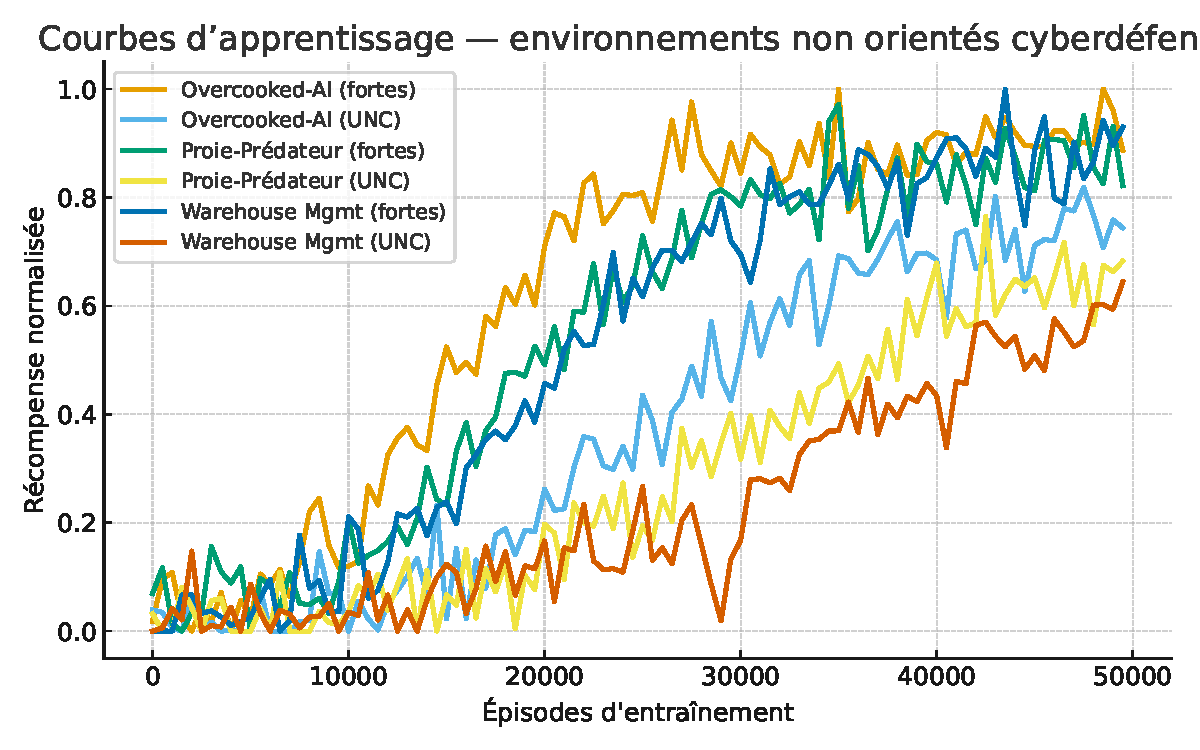
\includegraphics[trim=0cm 0cm 0cm 1cm, clip, width=0.8\linewidth]{figures/results_noncyber_learning.pdf}
        \vspace{-0.3cm}
        \caption*{{\scriptsize Learning curves}}
        \label{fig:noncyber_learning_curves}
      \end{figure}

    \end{column}

  \end{columns}

\end{frame}


\begin{frame}{Case Study}{Company Infrastructure~\parencite{cage-challenge-announcement}}

  \vspace{-0cm}

  \begin{columns}[c]

    \hspace{-0.5cm}

    \begin{column}{0.5\textwidth}

      \textbf{Three organizational models:}
      \begin{itemize}
        \item Random attacker / defender
        \item Manual attacker / defender
        \item Learning attacker / defender
      \end{itemize}


      \vspace{1cm}


      \begin{figure}

        \centering
        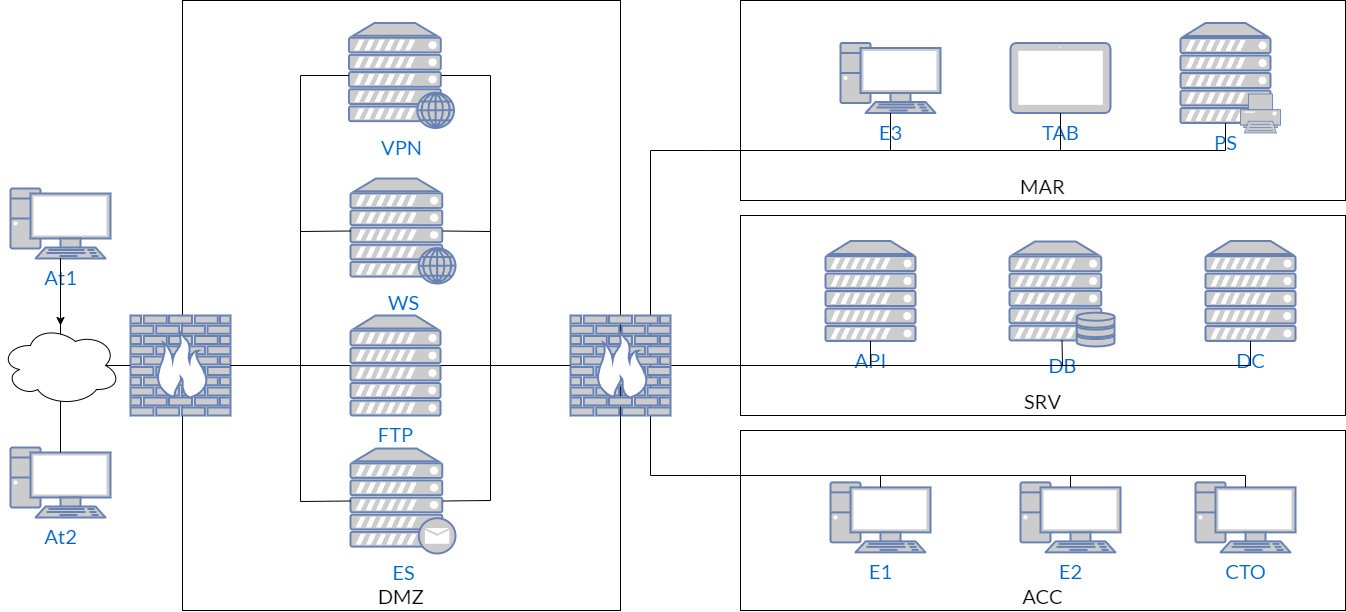
\includegraphics[width=0.8\linewidth]{figures/network_infra.png}
        \caption*{Topology of the small-scale company infrastructure.}
      \end{figure}

    \end{column}

    \hspace{-0.5cm}

    \begin{column}{0.5\textwidth}
      \hspace{1cm}

      \begin{figure}

        \centering
        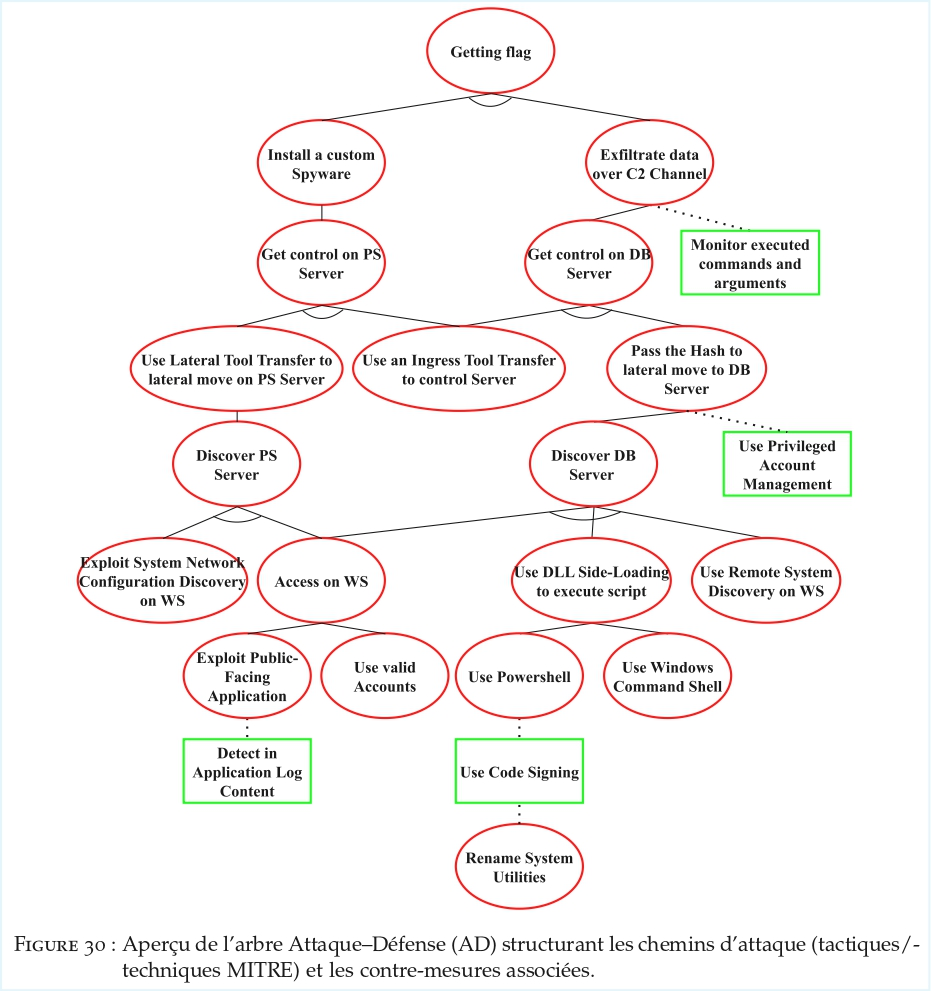
\includegraphics[trim=0.1cm 1.4cm 0.1cm 0.1cm, clip, width=0.8\linewidth]{figures/attack_defense_tree.jpg}
        \caption*{Attack-defense tree used in CAGE Challenge scenario no. 1~\parencite{cage-challenge-announcement}, based on \textbf{MITRE ATT\&CK}~\parencite{MITREATTACKWebiste}.}

      \end{figure}

    \end{column}

  \end{columns}


\end{frame}

% \begin{frame}{Etude de cas}{Infrastructure d'entreprise}

%   \vspace{-0.5cm}

%   \begin{columns}[c]

%     \hspace{-0cm}

%     \begin{column}{0.5\textwidth}
%       {\scriptsize
%         \textbf{Principaux résultats :}
%         \begin{itemize}

%           \item Modélisation
%                 \begin{itemize}
%                   \item Validé quand dataset de trajectoires \textquote{assez important} (>5 Go)
%                 \end{itemize}

%           \item Entrainement
%                 \begin{itemize}
%                   \item Validé vis-à-vis du respect des contraintes dures et douces (taux de violation 0 pour dureté de contraintes forte)
%                 \end{itemize}

%           \item Analyse
%                 \begin{itemize}
%                   \item Validé rôles et objectifs inférées correspondent aux attentes (vérification manuelle des trajectoires produites)
%                 \end{itemize}

%           \item Transfert
%                 \begin{itemize}
%                   \item Validé prise en compte des modifications environnementales en temps réel (ajout/retrait d'un nœud dans le réseau)
%                 \end{itemize}

%         \end{itemize}
%       }
%     \end{column}

%     \begin{column}{0.5\textwidth}
%       \centering
%       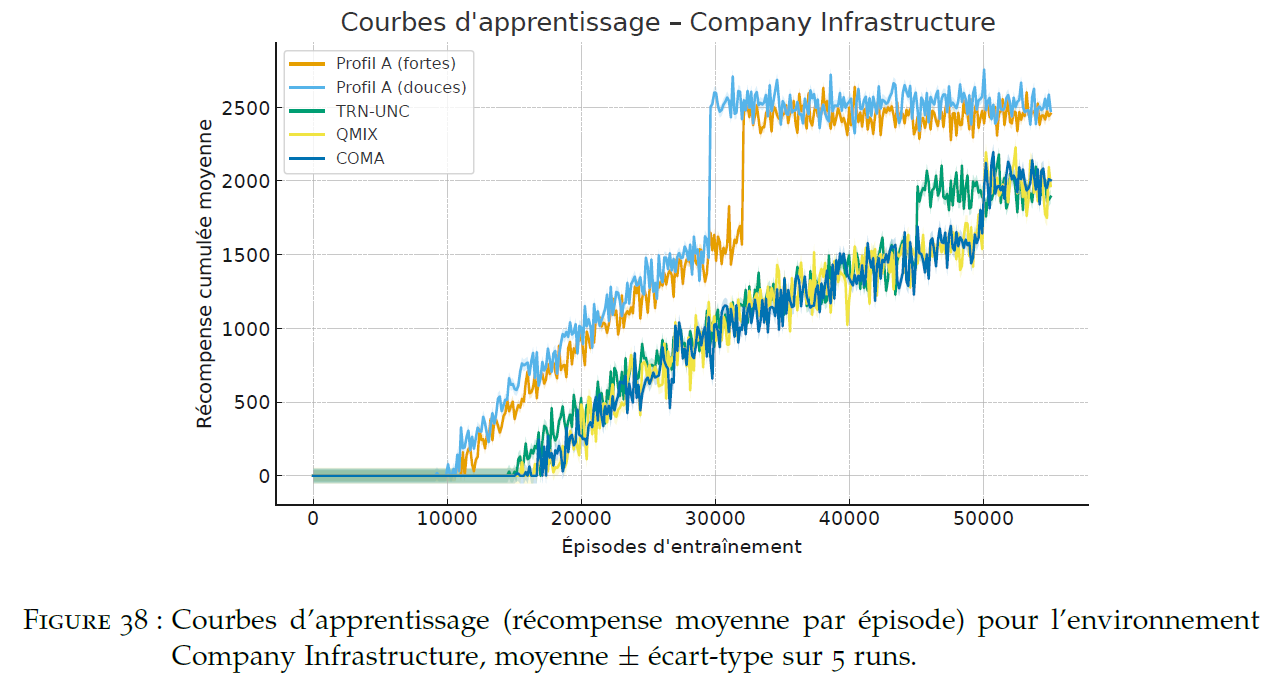
\includegraphics[width=1\linewidth]{figures/company_infra_learning_curve.png}
%       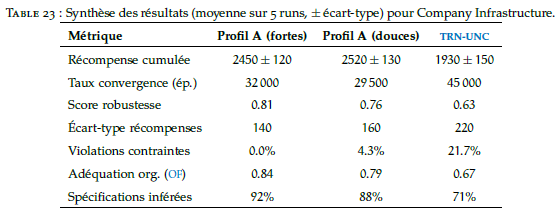
\includegraphics[width=0.9\linewidth]{figures/infra_results.png}
%       \vspace{-1cm}
%     \end{column}

%   \end{columns}

% \end{frame}


\begin{frame}{Case Study}{Drone Swarm Scenario~\parencite{cage_challenge_3_announcement}}

  \begin{columns}
    \begin{column}{0.5\textwidth}

      \textbf{Three organizational models:}
      \begin{itemize}
        \item \textquote{Suspect Isolation}
        \item \textquote{Active Defense}
        \item \textquote{Manual}
      \end{itemize}

      \hspace{1.5cm}
      \makebox[0.4\textwidth][c]{\animategraphics[loop,autoplay,scale=0.19]{8}{figures/cyborg/frame}{0}{33}}

    \end{column}


    \begin{column}{0.5\textwidth}

      \vspace{-0.2cm}
      \centering

      \begin{figure}
        \centering
        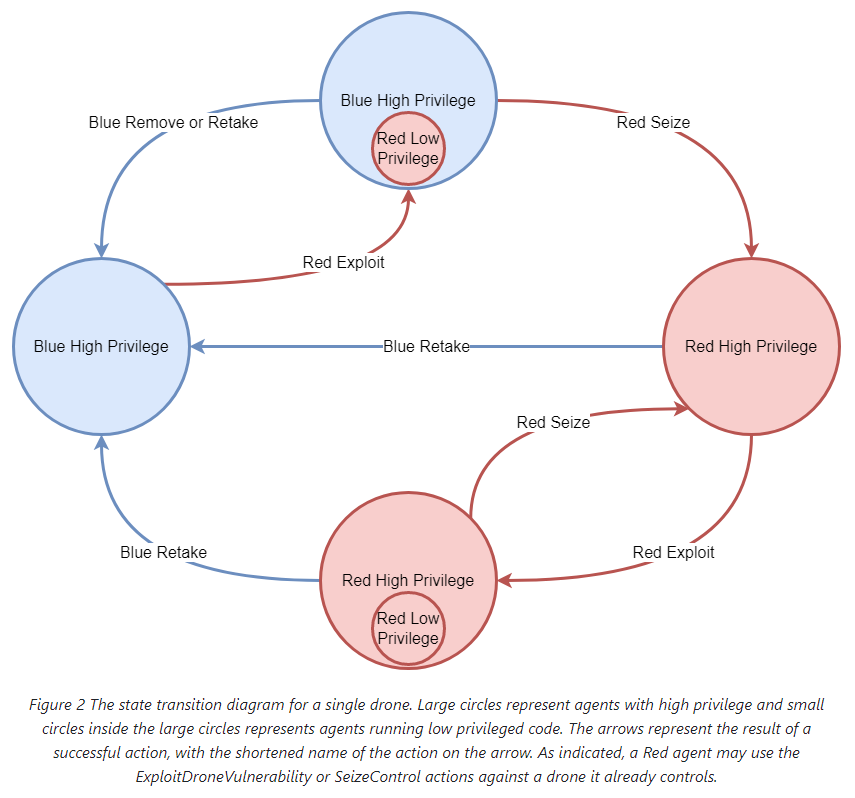
\includegraphics[trim=0cm 2.4cm 0cm 0.2cm, clip,width=0.65\linewidth]{figures/markov_mdp_drones.png}
        \caption*{State-transition diagram for a drone.}
      \end{figure}


      \vspace{-0.25cm}

      \begin{figure}
        \centering
        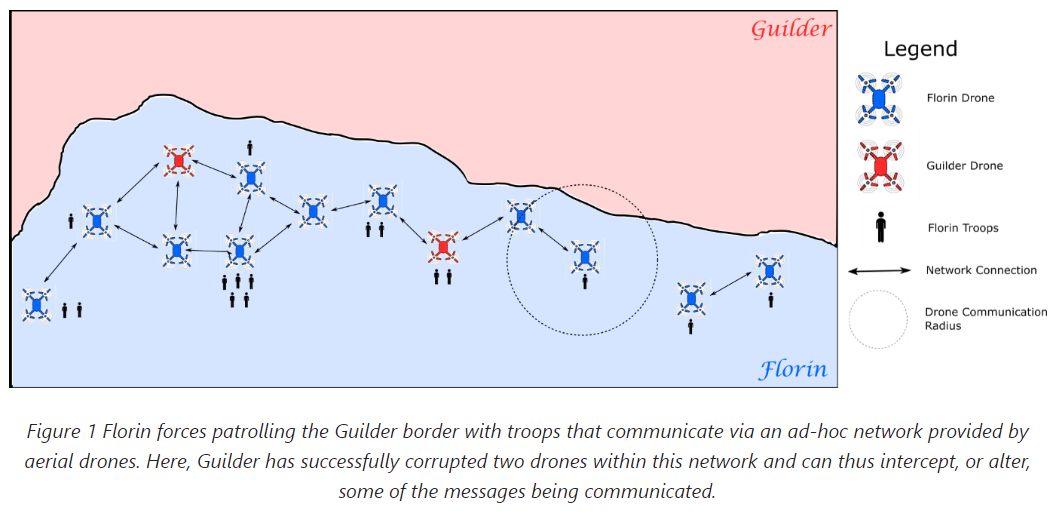
\includegraphics[trim=0cm 2cm 0cm 0cm, clip,width=0.6\linewidth]{figures/drones_illustration.png}
        \caption*{CAGE Challenge scenario no. 3~\parencite{cage_challenge_3_announcement}: protecting \textquote{benign} drones from \textquote{infected} drones.}
      \end{figure}

    \end{column}
  \end{columns}




\end{frame}

% \begin{frame}{Etude de cas}{Scénario essaim de drones}

%   \vspace{-0.5cm}

%   \begin{columns}[c]

%     \hspace{-0cm}

%     \begin{column}{0.5\textwidth}
%       {\scriptsize
%         \textbf{Principaux résultats :}
%         \begin{itemize}

%           \item Modélisation
%                 \begin{itemize}
%                   \item Validé quand dataset de trajectoires \textquote{assez important} (>5 Go)
%                 \end{itemize}

%           \item Entrainement
%                 \begin{itemize}
%                   \item Validé comme plus stable et plus grande convergence
%                 \end{itemize}

%           \item Analyse
%                 \begin{itemize}
%                   \item Validé rôles et objectifs inférées correspondent aux attentes (vérification manuelle des trajectoires produites)
%                 \end{itemize}

%           \item Transfert
%                 \begin{itemize}
%                   \item Validé prise en compte des modifications environnementales en temps réel (forcer un drone à être infecté pour déstabiliser)
%                 \end{itemize}

%         \end{itemize}
%       }
%     \end{column}

%     \begin{column}{0.5\textwidth}
%       \ \\ \ \\
%       \centering
%       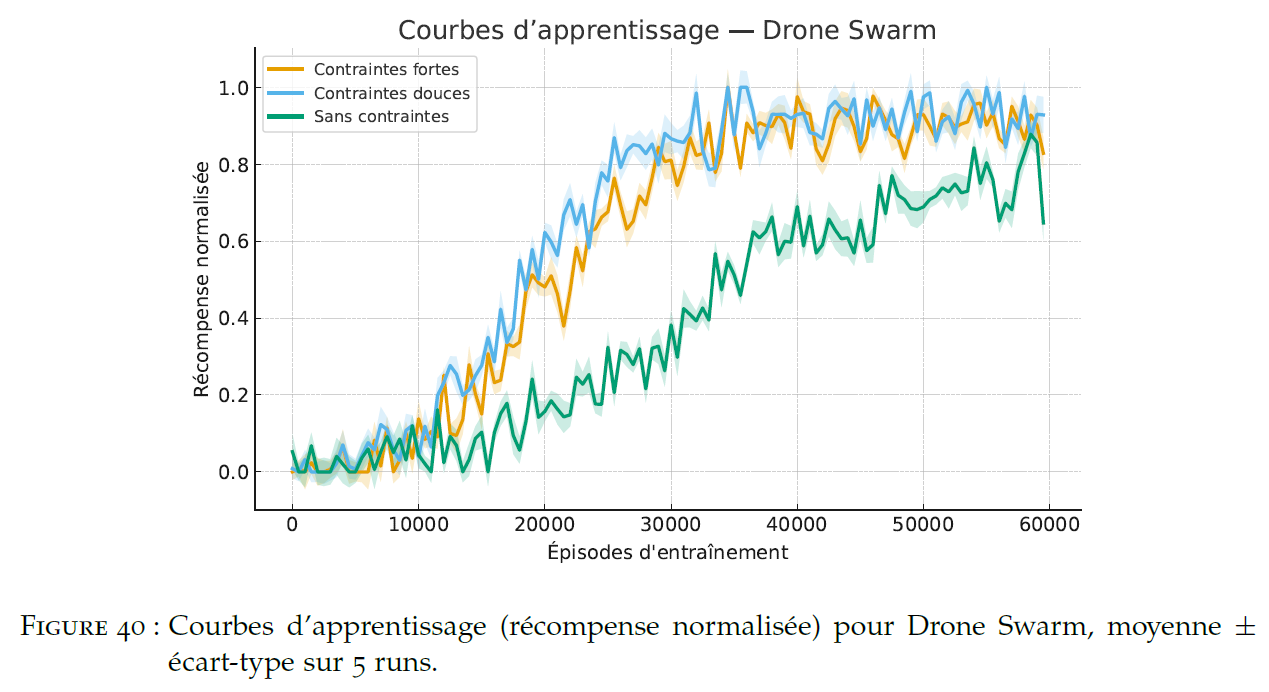
\includegraphics[width=0.87\linewidth]{figures/drone_swarm_results.png}
%       \ \\ \ \medskip
%       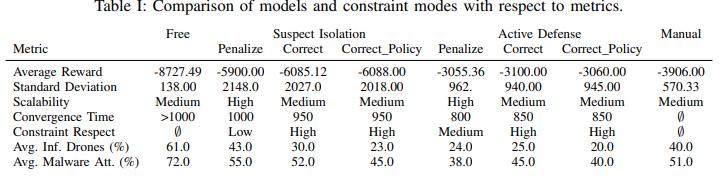
\includegraphics[width=0.87\linewidth]{figures/cage_own_results.png}
%       \ \\ \ \medskip
%       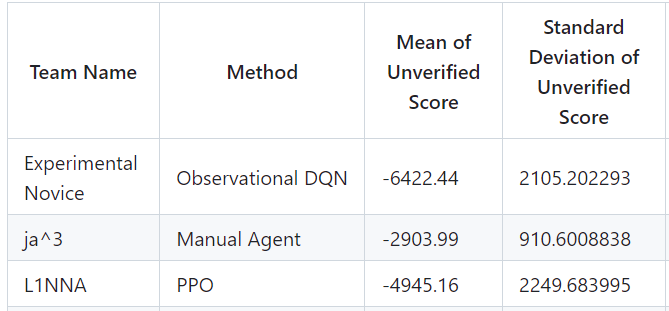
\includegraphics[width=0.5\linewidth]{figures/cage_leader_results.png}
%     \end{column}

%   \end{columns}

% \end{frame}


\begin{frame}{Case Study}{Kubernetes Microservices Architecture}

  \centering
  % 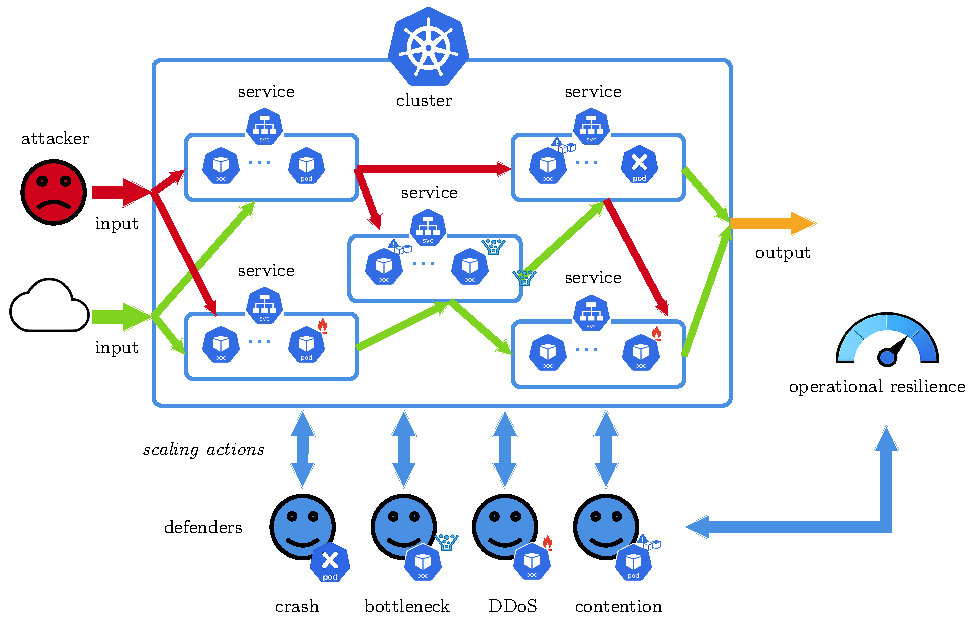
\includegraphics[width=0.7\linewidth]{figures/scenario_introduction.pdf}
  \resizebox{!}{0.8\textheight}{\input{figures/scenario_k8s.tex}}

  \vfill

  {\tiny \begin{spacing}{0.8}
      \textit{J. Soule, J.-P. Jamont, M. Occello, L.-M. Traonouez, and P. Théron. Streamlining Resilient Kubernetes Autoscaling with Multi-Agent Systems via an Automated Online Design Framework. Proceedings of the 18th IEEE International Conference on Cloud Computing (CLOUD), Helsinki, Finland, July 2025.}
    \end{spacing}}

\end{frame}

\begin{frame}{Case Study}{Kubernetes Microservices Architecture}


  \begin{columns}[c]

    \begin{column}{0.4\textwidth}

      \textbf{MAS approach}
      \begin{itemize}
        \item One agent per issue
        \item Target issues by priority
        \item Easier scaling
      \end{itemize}

      \

      \textbf{Implementation in KARMA (\textit{Kubernetes Autoscaling with Resilient Multi-Agent System})}
      \begin{itemize}
        \item Functional proof of concept on a simple cluster
        \item Improved operational resilience
        \item Faster convergence
      \end{itemize}

    \end{column}

    \begin{column}{0.7\textwidth}

      \resizebox{1\linewidth}{!}{\input{figures/karma_architecture/karma_architecture.tex}}

    \end{column}
  \end{columns}

  \vfill

  {\tiny \begin{spacing}{0.8}
      \textit{J. Soule, J.-P. Jamont, M. Occello, L.-M. Traonouez, and P. Théron. Streamlining Resilient Kubernetes Autoscaling with Multi-Agent Systems via an Automated Online Design Framework. Proceedings of the 18th IEEE International Conference on Cloud Computing (CLOUD), Helsinki, Finland, July 2025.}
    \end{spacing}}

\end{frame}

% \begin{frame}{Étude de cas}{Architecture des microservices Kubernetes}

%   \vspace{-0cm}

%   \begin{columns}[c]

%     \hspace{-0cm}

%     \begin{column}{0.5\textwidth}
%       {\scriptsize
%         \textbf{Principaux résultats :}
%         \begin{itemize}

%           \item Modélisation
%                 \begin{itemize}
%                   \item Validé quand dataset de trajectoires \textquote{assez important} (>7 Go)
%                 \end{itemize}

%           \item Entrainement
%                 \begin{itemize}
%                   \item Validé comme plus stable, plus grande convergence, résilience opérationnelle plus importante que HPA
%                 \end{itemize}

%           \item Analyse
%                 \begin{itemize}
%                   \item Validé rôles et objectifs inférées correspondent aux attentes (vérification manuelle des trajectoires produites, visualisation PCA…)
%                 \end{itemize}

%           \item Transfert
%                 \begin{itemize}
%                   \item Validé prise en compte des modifications environnementales en temps réel (changement brusque du volume d'entrée, changement politique de l'attaquant…)
%                 \end{itemize}

%         \end{itemize}
%       }
%     \end{column}

%     \begin{column}{0.5\textwidth}
%       \centering
%       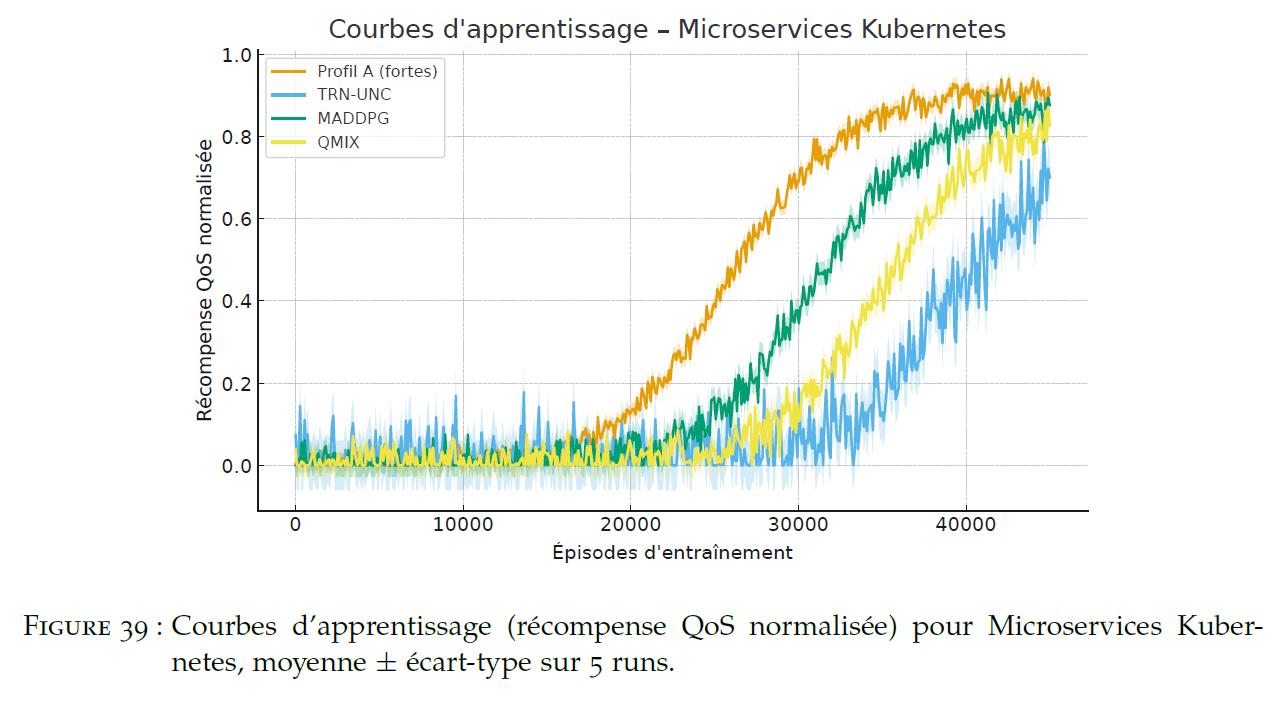
\includegraphics[width=0.87\linewidth]{figures/k8s_learning_curve.png}
%       \ \\ \ \medskip
%       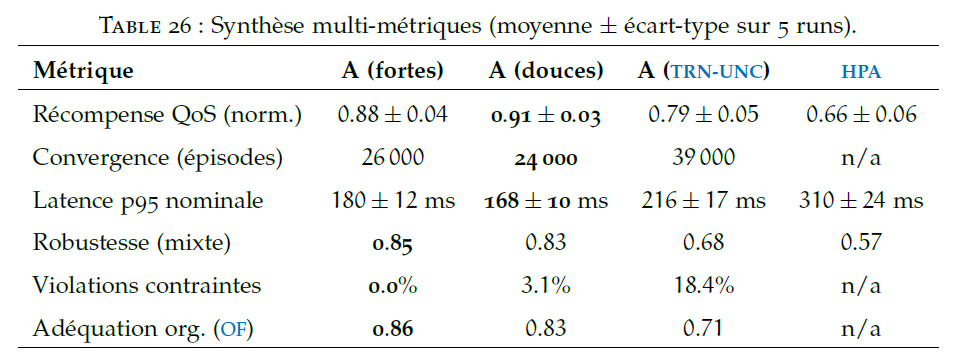
\includegraphics[width=0.87\linewidth]{figures/k8s_results.png}
%     \end{column}

%   \end{columns}

%   \vfill

%   {\tiny \begin{spacing}{0.8}
%       \textit{J. Soule, J.-P. Jamont, M. Occello, L.-M. Traonouez, and P. Théron. Streamlining Resilient Kubernetes Autoscaling with Multi-Agent Systems via an Automated Online Design Framework. Proceedings of the 18th IEEE International Conference on Cloud Computing (CLOUD), Helsinki, Finland, July 2025.}
%     \end{spacing}}

% \end{frame}

\begin{frame}{Selected Results for Cyber-Defense Environments (1/2)}

  \begin{columns}
    \begin{column}{0.6\textwidth}
      \vspace{-0.5cm}

      \begin{table}[h!]
        \centering
        \caption*{Summary of results for \textit{Company Infrastructure}.}
        \vspace{-0.1cm}
        \label{tab:infra_results}
        \renewcommand{\arraystretch}{1.2}
        \small

        \resizebox{1\linewidth}{!}{

          \begin{tabular}{lccc}
            \hline
            \textbf{Metric}                  & \textbf{Profile A (hard)} & \textbf{Profile A (soft)} & \textbf{\textbf{TRN-UNC}} \\
            \hline
            Cumulative reward                & $2450 \pm 120$            & $2520 \pm 130$            & $1930 \pm 150$            \\
            Convergence rate (ep.)           & $32\,000$                 & $29\,500$                 & $45\,000$                 \\
            Robustness score                 & $0.81$                    & $0.76$                    & $0.63$                    \\
            Reward standard deviation        & $140$                     & $160$                     & $220$                     \\
            Constraint violations            & $0.0\%$                   & $4.3\%$                   & $21.7\%$                  \\
            Organizational fit (\textbf{OF}) & $0.84$                    & $0.79$                    & $0.67$                    \\
            Inferred specifications          & $92\%$                    & $88\%$                    & $71\%$                    \\
            \hline
          \end{tabular}}
      \end{table}

      \vspace{-0.1cm}

      \begin{figure}
        \centering
        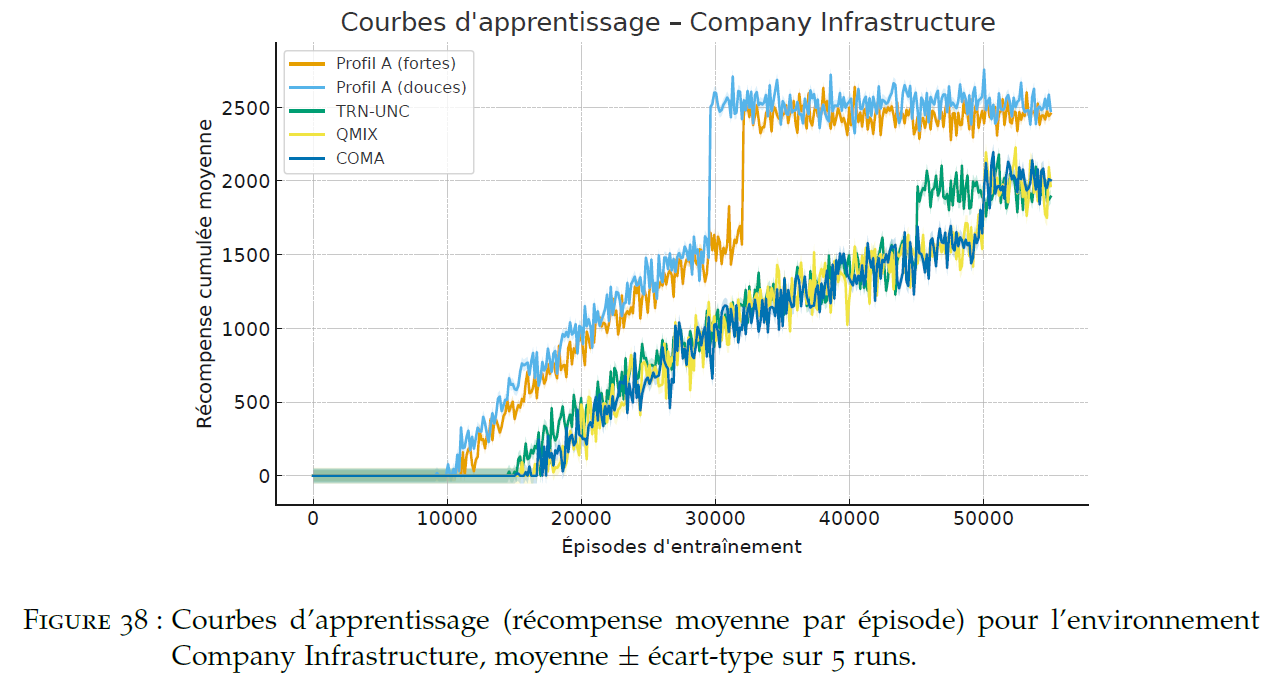
\includegraphics[trim={4cm 2.8cm 0cm 0.8cm},clip,width=0.9\linewidth]{figures/company_infra_learning_curve.png}
        \vspace{-0.1cm}
        \caption*{Learning curves for \textit{Company Infrastructure}.}
      \end{figure}

    \end{column}

    \begin{column}{0.4\textwidth}
      \begin{itemize}
        \item Convergence, stationarity, stability
        \item Robustness
        \item Constraint compliance
        \item Performance
        \item Explainability
      \end{itemize}
    \end{column}
  \end{columns}



\end{frame}

\begin{frame}{Selected Results for Cyber-Defense Environments (2/2)}

  \begin{columns}

    \begin{column}{0.5\textwidth}
      \centering
      \vspace{-0.5cm}

      \begin{table}[t]
        \centering
        \setlength{\tabcolsep}{4.5pt}
        \caption*{Comparison of constraint baselines for \textit{Drone Swarm} against participant results.}
        \label{tab:metrics_comparison}

        \resizebox{1\linewidth}{!}{
          \begin{tabular}{lcccccccccccc}
                                   & {Free}      & \multicolumn{3}{c}{Suspect Isolation} & \multicolumn{3}{c}{Active Defense} & {Manual}                                                              \\
            % \cline{2-13}
            Metric                 &             & Penalize                              & Correct                            & Correct\_Policy & Penalize & Correct  & Correct\_Policy &             \\
            \midrule
            Average Reward         & -8727.49    & -5900.00                              & -6085.12                           & -6088.00        & -3055.36 & -3100.00 & -3060.00        & -3906.00    \\
            Standard Deviation     & 138.00      & 2148.0                                & 2027.0                             & 2018.00         & 962.     & 940.00   & 945.00          & 570.33      \\
            Scalability            & Medium      & High                                  & Medium                             & Medium          & High     & Medium   & Medium          & Medium      \\
            Convergence Time       & >1000       & 1000                                  & 950                                & 950             & 800      & 850      & 850             & $\emptyset$ \\
            Constraint Respect     & $\emptyset$ & Low                                   & High                               & High            & Medium   & High     & High            & $\emptyset$ \\
            Avg. Inf. Drones (\%)  & 61.0        & 43.0                                  & 30.0                               & 23.0            & 24.0     & 25.0     & 20.0            & 40.0        \\
            Avg. Malware Att. (\%) & 72.0        & 55.0                                  & 52.0                               & 45.0            & 38.0     & 45.0     & 40.0            & 51.0        \\
            \hline
          \end{tabular}}
      \end{table}

      \vspace{0.5cm}

      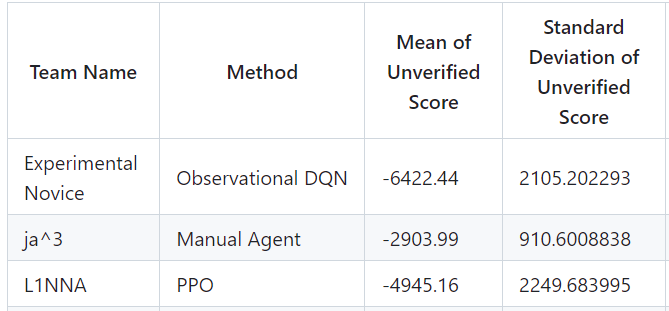
\includegraphics[width=0.8\linewidth]{figures/cage_leader_results.png}

    \end{column}

    \begin{column}{0.5\textwidth}
      \centering

      \begin{table}[h!]
        \centering
        \caption*{Multi-metric summary for the \textit{Microservices K8s} environment.}
        \label{tab:k8s_summary}
        \renewcommand{\arraystretch}{1.2}
        \small
        \vspace{-0.5cm}
        \resizebox{1\linewidth}{!}{
          \begin{tabular}{lcccc}
            \hline
            \textbf{Metric}                  & \textbf{A (hard)} & \textbf{A (soft)}        & \textbf{A (\textbf{TRN-UNC})} & \textbf{\textbf{HPA}} \\
            \hline
            Normalized QoS reward            & $0.88 \pm 0.04$   & $\mathbf{0.91 \pm 0.03}$ & $0.79 \pm 0.05$               & $0.66 \pm 0.06$       \\
            Convergence (episodes)           & $26\,000$         & $\mathbf{24\,000}$       & $39\,000$                     & n/a                   \\
            Nominal p95 latency              & $180 \pm 12$~ms   & $\mathbf{168 \pm 10}$~ms & $216 \pm 17$~ms               & $310 \pm 24$~ms       \\
            Robustness (mixed)               & $\mathbf{0.85}$   & $0.83$                   & $0.68$                        & $0.57$                \\
            Constraint violations            & $\mathbf{0.0\%}$  & $3.1\%$                  & $18.4\%$                      & n/a                   \\
            Organizational fit (\textbf{OF}) & $\mathbf{0.86}$   & $0.83$                   & $0.71$                        & n/a                   \\
            \hline
          \end{tabular}}
      \end{table}

      \vspace{1cm}

      \begin{itemize}
        \item Convergence, stationarity, stability
        \item Robustness
        \item Constraint compliance
        \item Performance
        \item Explainability
      \end{itemize}
    \end{column}


  \end{columns}



\end{frame}

\begin{frame}{Overall Coverage of Criteria C1--C5}
  \scriptsize
  \setlength{\tabcolsep}{8pt}
  \renewcommand{\arraystretch}{1.5}
  \setlength{\extrarowheight}{2pt}
  \centering
  \begin{tabular}{lccccc}
    \hline
    \textbf{Environment}   & \textbf{C1 Autonomy} & \textbf{C2 Performance} & \textbf{C3 Adaptation} & \textbf{C4 Control} & \textbf{C5 Explainability} \\
    \hline
    Overcooked-AI          & 0.20                 & 0.82                    & 0.80                   & 0.75                & 0.72                       \\
    Predator-Prey          & 0.20                 & 0.79                    & 0.77                   & 0.73                & 0.69                       \\
    Warehouse Management   & 0.20                 & 0.85                    & 0.82                   & 0.77                & 0.76                       \\
    Company Infrastructure & 0.25                 & 0.88                    & 0.83                   & 0.85                & 0.81                       \\
    Microservices K8s      & 0.25                 & 0.91                    & 0.86                   & 0.88                & 0.83                       \\
    Drone Swarm            & 0.20                 & 0.89                    & 0.84                   & 0.86                & 0.82                       \\
    \hline
    \textbf{Average}       & \textbf{0.21}        & \textbf{0.86}           & \textbf{0.82}          & \textbf{0.81}       & \textbf{0.77}              \\
    \hline
  \end{tabular}

  \vspace{0.6em}
  \begin{itemize}\scriptsize
    \item \textbf{Increased stability}: a marked reduction in inter-episode variance $\Rightarrow$ more stable learning and more readable behaviors.
    \item \textbf{Control}: constraint violation rate $<1\,\%$, with role and mission consistency preserved across all environments.
    \item \textbf{Explainability}: mean alignment $\approx 0.8$ between inferred roles and $\mathcal{M}OISE^+$ specifications $\Rightarrow$ automated post-hoc understanding.
    \item \textbf{Adaptation}: robustness confirmed under agent failures, node addition/removal, and topology changes.
    \item \textbf{Non-stationarity}: faster convergence, more stable policies, and higher cumulative rewards across the use cases.
  \end{itemize}
\end{frame}


\section{Conclusion}

\begin{frame}{}
  \tableofcontents[currentsection]
\end{frame}

\begin{frame}{Summary of Contributions, Benefits, and Improvement Axes}

  \small

  \begin{table}[h]

    \centering
    \setlength{\tabcolsep}{8pt}
    \renewcommand{\arraystretch}{1.7}
    % \setlength{\extrarowheight}{2pt}

    \resizebox{0.95\textwidth}{!}{
      \begin{tabular}{cp{6.5cm}p{6.5cm}}
        \textbf{Contributions} & \textbf{Benefits}                                      & \textbf{Improvement Axes}                                          \\
        \hline                                                                                                                                               \\[-2mm]

        % --- MAMAD (4 lignes) ---
        \multirow{3}{5.2cm}{\textbf{MAMAD framework}                                                                                                         \\(MOD -- TRN -- ANL -- TRF)}
                               & $\bullet$ Unified vision                               & $\bullet$ Methodological refinement                                \\
                               & $\bullet$ End-to-end pipeline $\rightarrow$ automation & $\bullet$ Stronger automation principles                           \\
                               & $\bullet$ Symbolic $\leftrightarrow$ learning          &                                                                    \\[1mm]
        \hdashline
        % --- World Models (3 lignes apports / 3 axes) ---
        \multirow{3}{5.2cm}{\textbf{Multi-agent World Models}                                                                                                \\(joint dynamics)}
                               & $\bullet$ Multi-agent prediction                       & $\bullet$ Scalability                                              \\
                               & $\bullet$ Adaptive digital twin                        & $\bullet$ Management of heterogeneous environments                 \\
                               &                                                        & $\bullet$ Data dependence                                          \\[1mm]
        \hdashline
        % --- $\mathcal{M}OISE^+$ / MARL (3 lignes) ---
        \multirow{3}{5.2cm}{\textbf{$\mathcal{M}OISE^+$ / MARL integration}}
                               & $\bullet$ Constraint-aware learning                    & $\bullet$ Goal prioritization in \textit{reward shaping}           \\
                               & $\bullet$ Robustness \& collective consistency         & $\bullet$ Adaptation to dynamic organizations                      \\
                               & $\bullet$ Roles/goals $\leftrightarrow$ policies       & $\bullet$ Individual guarantee $\rightarrow$ collective guarantee  \\[1mm]
        \hdashline
        % --- TEMM (2 lignes) ---
        \multirow{2}{5.2cm}{\textbf{Organizational analysis}                                                                                                 \\(TEMM)}
                               & $\bullet$ Explainability through roles \& goals        & $\bullet$ Stronger automation                                      \\
                               & $\bullet$ Validation of emergent roles                 & $\bullet$ Causal / logical analysis (plans in $\mathcal{M}OISE^+$) \\[1mm]
        \hdashline
        % --- Transfert / sim2real (2 lignes) ---
        \multirow{2}{5.2cm}{\textbf{Transfer through a digital twin}}
                               & $\bullet$ Reduced sim-to-real gap                      & $\bullet$ Multi-platform validation                                \\
                               & $\bullet$ Model $\leftrightarrow$ policy loop          & $\bullet$ Calibration under real-time fluctuations                 \\[1mm]
        \hdashline
        % --- CybMASDE (3 lignes) ---
        \multirow{3}{5.2cm}{\textbf{CybMASDE platform}}
                               & $\bullet$ Unified architecture                         & $\bullet$ Performance optimization                                 \\
                               & $\bullet$ Modularity \& genericity                     & $\bullet$ Broader RL interoperability                              \\
                               & $\bullet$ Automation / assistance (\textit{HPO})       & $\bullet$ Integration with existing tools
        \\
        \hline
      \end{tabular}}
  \end{table}

\end{frame}


\begin{frame}{Perspectives and Extensions}
  \small
  \textbf{Short- and medium-term directions}
  \begin{itemize}
    \item \textbf{Richer modeling}: hybridization of data and expert knowledge (\textit{neuro-symbolic World Model});
    \item \textbf{More robust learning}: dynamic environments, adaptive adversaries, continuous Sim2Real;
    \item \textbf{Integration of \textquote{$\mathcal{M}OISE^+$ goal plans}} into learning $\rightarrow$ challenging prioritization issues;
    \item \textbf{Advanced analysis}: inference of roles, goals, and plans, role inheritance, etc. (\textbf{ML} and \textbf{LLM}).
  \end{itemize}

  \vspace{1cm}
  \textbf{Longer-term challenges}
  \begin{itemize}
    \item \textbf{Scalability}: distributed MAS on real networks
    \item \textbf{Operational interoperability}: integration with SOC / CSIRT settings
    \item \textbf{Human acceptability and explainability}: transparency, auditability, trust
  \end{itemize}

  \vspace{0.3em}
  \centering
  \textit{\textbf{$\rightarrow$ Toward autonomous, safe, and understandable MAS in real environments.}}
\end{frame}


\section*{\phantom{X}}

\miniframesoff

\input{sections/thanks}

% \useoutertheme{miniframes}

% \section*{Publications et communications}

\begin{frame}{Publications and Communications}{}
  \scriptsize

  \textbf{International journal}
  \begin{itemize}
    \item Soulé, J., Jamont, J.-P., Occello, M., Traonouez, L.-M., Théron, P.
          \textit{Assisting Multi-Agent System Design with $\mathcal{M}OISE^+$ and MARL: The MAMAD Method}.
          \textbf{JAAMAS}, 2025 (under review).
  \end{itemize}

  \vspace{0.6em}

  \textbf{International conferences}
  \begin{itemize}
    \item Soulé, J., Jamont, J.-P., Occello, M., Traonouez, L.-M., Théron, P.
          \textit{An Organizationally-Oriented Approach to Enhancing Explainability and Control in Multi-Agent Reinforcement Learning}.
          \textbf{AAMAS} 2025, Detroit, USA.

    \item Soulé, J., Jamont, J.-P., Occello, M., Traonouez, L.-M., Théron, P.
          \textit{Streamlining Resilient Kubernetes Autoscaling with Multi-Agent Systems via an Automated Online Design Framework}.
          IEEE \textbf{CLOUD} 2025, Helsinki.

    \item Soulé, J., Jamont, J.-P., Occello, M., Traonouez, L.-M., Théron, P.
          \textit{A MARL-Based Approach for Easing MAS Organization Engineering}.
          \textbf{AIAI} 2024 (Springer LNCS).

    \item Soulé, J., Jamont, J.-P., Occello, M., Théron, P., Traonouez, L.-M.
          \textit{Towards a Multi-Agent Simulation of Cyber-Attackers and Cyber-Defenders Battles}.
          IEEE \textbf{SMC} 2023.
  \end{itemize}

  \vspace{0.6em}

  \textbf{National conferences}
  \begin{itemize}
    \item Soulé, J., Jamont, J.-P., Occello, M., Théron, P., Traonouez, L.-M.
          \textit{Une approche organisationnelle pour améliorer l'explicabilité et le contrôle dans l'apprentissage par renforcement multi-agent}.
          \textbf{JFSMA} 2025 — \textbf{Best Paper Award}.

    \item Soulé, J., Jamont, J.-P., Occello, M., Traonouez, L.-M., Théron, P.
          \textit{Une approche basée sur l'apprentissage par renforcement pour l'ingénierie organisationnelle d'un SMA}.
          \textbf{JFSMA} 2024.
    \item Soulé, J., Jamont, J.-P., Occello, M., Traonouez, L.-M., Théron, P.
          \textit{Un outil pour la conception de SMA par apprentissage par renforcement et modélisation organisationnelle}.
          \textbf{JFSMA} 2024.

    \item Soulé, J., Jamont, J.-P., Occello, M., Théron, P., Traonouez, L.-M.
          \textit{De l'organisation d'un système multi-agent de Cyberdéfense}.
          \textbf{RESSI} 2023.
    \item Soulé, J., Jamont, J.-P., Occello, M., Théron, P., Traonouez, L.-M.
          \textit{De l'organisation d'un système multi-agent de Cyberdéfense}.
          \textbf{RJCIA} 2023.

  \end{itemize}

\end{frame}

% \useoutertheme{miniframes}

\section*{\phantom{References}}
\begin{frame}[allowframebreaks]{References}{}
  \printbibliography[heading=none]
\end{frame}

\miniframeson

\appendix

\newcounter{mainframenumber}
\setcounter{mainframenumber}{\value{framenumber}}

\input{sections/annexes}


\end{document}
